\documentclass[a4paper,14pt,oneside]{book}
\usepackage[utf8]{inputenc}
\usepackage[a4paper, inner=3cm,outer=2cm,top=1.5cm,bottom=1.5cm]{geometry}
\usepackage{makeidx}
\usepackage{amsmath,amsfonts,amssymb,amsthm,epsfig,epstopdf,titling,url,array,bm}
\usepackage{sectsty}
\usepackage{pdflscape}
\usepackage{makeidx}
\makeindex
\usepackage{rotating}
\usepackage[toc,page]{appendix}
\usepackage{makecell}
\usepackage[dvipsnames]{xcolor}
\usepackage{tikz}
\usepackage{csquotes}
\usepackage{afterpage}
\usepackage{capt-of}
\usepackage{tcolorbox}
\usepackage{pgffor}
\usepackage{tikz}
\usepackage{pifont}
\usepackage[document]{ragged2e}
\usepackage[bookmarks,bookmarksnumbered]{hyperref}
\usepackage{enumitem}
\setlength{\parindent}{2em}
\setlength{\parskip}{1em}
\renewcommand{\baselinestretch}{1.4}
\theoremstyle{plain}
\newtheorem{thm}{Theorem}[section]
\newtheorem{lem}[thm]{Lemma}
\newtheorem{prop}[thm]{Proposition}
\newtheorem{cor}{Corollary}[thm]
\theoremstyle{definition}
\newtheorem{defn}{Definition}[section]
\newtheorem{conj}{Conjecture}[section]
\newtheorem{exmp}{Example}[section]%\theoremstyle{table}
\newtheorem{tab}{Table}[section]%\theoremstyle{caption}
\newtheorem{capt}{Table}[section]
\theoremstyle{remark}
\newtheorem{rmk}{Remark}[section]
\newtheorem*{note}{Note}
\pagenumbering{arabic}
\setcounter{tocdepth}{5}
\begin{document}
\begin{titlepage}
\begin{center}
\vspace*{0.3cm}
\huge
\textbf{\color{blue!70!green}D. B. F. Dayanand College of Arts and Science, Solapur}\\
\vspace{0.1cm}
\includegraphics[scale=0.4]{College}\\
\Large{
\textcolor{red}{A Project Report} \\ \textcolor{blue}{on}}\\
\vspace{0.5cm}\textcolor{purple}{\Huge {\textbf{Introduction to Fractional Calculus}}}\\
\textcolor{green!30!blue}{Presented by} \\\textbf{\textcolor{Orchid!150!}{Mr. Tatipamul Jayesh Ravimohan ( Roll No: 7376 ) \\ Mr. Bharale Shriniwas Suresh ( Roll No: 7375 ) \\ Mr. Bussa Mohan Ashok ( Roll No: 7378 ) \\  Mr. Bulla Shridhar Shivanand ( Roll No: 7360 )}}\\\huge{\textbf{\textcolor{magenta}{M.Sc. Part-II}}}\\
\textbf{\textcolor{cyan}{UNDER THE GUIDANCE OF}}\\
\textcolor{teal}{\textit {\textbf{Shri. Anand R. Reshimkar}}}\\
\textcolor{violet}{submitted to}\\
\textbf{\textcolor{red}{\LARGE{DEPARTMENT OF MATHEMATICS}}}\\
\textcolor{purple}{\textsc{D. B. F. Dayanand College of Arts and Science, Solapur}}\\
\textcolor{blue}{P. A. H. SOLAPUR UNIVERSITY, SOLAPUR}

\newpage
\vspace*{4cm}
\begin{center}
\textbf{DECLARATION}  \\
\justify
\Large{
We, Mr. Tatipamul Jayesh Ravimohan, Mr. Bharale Shriniwas Suresh, Mr. Bussa Mohan Ashok and Mr. Bulla Shridhar Shivanand, the students of M.Sc.II (Semester-IV) Mathematics, hereby declare that we have successfully completed this project on \textbf{\enquote{Introduction to Fractional Calculus}} in the academic year 2021-2022. The information in this project is true to the best of our knowledge.\\\flushleft Mr. Tatipamul Jayesh Ravimohan \hfill Mr. Bharale Shriniwas Suresh\\ 
\vspace{1.5cm}\flushleft Mr. Bussa Mohan Ashok  \hfill Mr. Bulla Shridhar Shivanand \\
\vspace{5.5cm}
\flushleft{Date :\hspace{0.8cm}/ \hspace{0.5cm} / }\hspace{8cm} Place: Solapur}
\end{center}

\newpage
\begin{center}
\huge{Department of Mathematics}\\[1cm]
\normalsize
\textsc{\Large{D. B. F. Dayanand College of Arts and Science, Solapur}}\\[2.0cm]
\textbf{\Large CERTIFICATE}\\
\end{center}
\Large
\justify
This is to certify that Mr. Tatipamul Jayesh Ravimohan, Mr. Bharale Shriniwas Suresh, Mr. Bussa Mohan Ashok and Mr. Bulla Shridhar Shivanand students of the Department of Mathematics, D. B. F. Dayanand College of Arts and Science, Solapur has undertaken the project on \textbf{\enquote{Introduction to Fractional Calculus}} during semester-IV of the academic year 2021-2022. This data collection and analysis of work for preparing the project has been carried out by the students from this college under P. A. H. Solapur University, Solapur under the guidance of Shri. Anand R. Reshimkar.\\
\indent I am satisfied with the work of  Mr. Tatipamul Jayesh Ravimohan,  Mr. Bharale Shriniwas Suresh, Mr. Bussa Mohan Ashok and Mr. Bulla Shridhar Shivanand.\\
\vfill
\begin{minipage}{3in}
Shri. Anand R. Reshimkar\\\hspace{1.6cm}Project Guide 
\end{minipage}\hspace{2cm}
\begin{minipage}{3in}
Shri. Anand R. Reshimkar\\\hspace{1.6cm}Coordinator
\end{minipage}
\vspace*{3cm}
\begin{center}
\hspace{1.1cm}External Examiner \hspace*{5.2cm} External Examiner
\end{center}

\newpage
\vspace*{4cm}
\begin{center}\textbf{Acknowledgement}
\end{center}\justify
\Large{
This gives us immense pleasure to produce this project report. We thank all faculties of the department, our project guide Shri. Anand R. Reshimkar for continuous guidance and support. We also thank each other in the group for their assistance.\\
\begin{flushright}
Mr. Tatipamul Jayesh Ravimohan \\
Mr. Bharale Shriniwas Suresh \\
Mr. Bussa Mohan Ashok \\
Mr. Bulla Shridhar Shivanand \\
\end{flushright}}

\newpage
\vspace{5cm}
\centering
\Huge
\textbf{\newline\ Introduction to Fractional Calculus}
\vfill
\today
\end{center}
\end{titlepage}

\begin{center}
\vspace*{4cm}
\huge{Abstract}\\
\justify
\Large{
In this report, the reader will not find a study of any kind; there is no
methodology, questionnaire, interview, test, or data analysis. This report is simply a report on fractional derivatives, a topic that I have found to be fascinating. The reader should be delighted by a short history of the topic in Chapter 1, where he/she will read about the contributions made by some of the great mathematicians from the last three centuries. In Chapter 2, we see an elementary introduction about Gamma, Beta and Mittag-Leffler functions and their various representations. Some of its most important properties are described. In Chapter 3, we look at the Riemann-Liouville fractional derivatives and its properties. The Caputo fractional derivative is discussed in more detail in chapter 4. A comparison with the Riemann-Liouville fractional derivative is made and a proof of an important relation formula that appears in the paper of Gorenflo and Mainardi \cite{bb18} without a proof, between these two derivatives, is deduced. As a corollary, the Leibniz rule for the Caputo operator is also derived. Some interesting examples of Caputo fractional derivatives of arbitrary constant,
power, exponential, sine and cosine functions are studied in Chapter 5. Proofs for the
general formulas are provided that cannot be found in the literature. Some special cases
are visualized by drawing graphs. All the results are summarized in a special chart. }
\end{center}

\Large{\tableofcontents}
\newpage
         
         \vspace{1cm} \chapter{History of Fractional Derivatives}
         \section{Leibniz 1690's}
         \begin{center}
         \begin{flushleft} 
         \justify
         \Large{
\par{The origin of fractional derivatives is not certain at this time, but we do know that Leibniz, the inventor of the notation $d^{n} y / dx^{n}$, had \textquotedblleft toyed\textquotedblright ~with the idea in the 1600's. In 1695 L'Hopital asked Leibniz: \textquotedblleft What if $n$ be 1/2?\textquotedblright ~Surprisingly Leibniz \cite{bb1} replied: \enquote{...You can see by that, sir, that one can express by an infinite series a quantity such as $d^{1 / 2} x y$ or $d^{1:2}x y$. Although infinite series and geometry are distant relations, infinite series admits only the use of exponents that are positive and negative integers, and does not, as yet, know the use of fractional exponents...} As with most great mathematicians, Leibniz had a unique insight into the unknown. He stumbled onto fractional derivatives realizing that one-day great things will come from his work. What they would be, he had no idea. In the same letter he continued: \enquote{... Thus it follows that $d^{1 / 2} x$ will be equal to $x \sqrt{dx: x}$. This is an apparent paradox from which, one day, useful consequences will be drawn...} Leibniz insight did not stop there. Three years latter in a letter to John Wallis, he discussed ways of using fractional derivatives in Wallis's infinite product for $1 / 2 \pi$. He states \cite{bb2}: \enquote{... Differential calculus might have been used to achieve this result...} It should be evident that Leibniz did not have just a passing thought on fractional derivatives, he must have spent a considerable amount of time on the topic. I wish I were a fly on the wall in the 1600's.}}
\end{flushleft}        \end{center}

\section{Euler 1738}
         \begin{center}
         \begin{flushleft} 
         \justify
         \Large{
\par{Euler, another great mathematician, toyed with the idea of fractional derivatives. 43 years after Leibniz went public with his controversial ideas of fractional derivatives,
Euler stated in his 1738 dissertation \cite{bb3} : \enquote{... When $n$ is a positive integer, and if $p$ should be a function of $x$, the ratio $d^{n} p$ to $d x^{n}$ can always be expressed algebraically, so that if $n=$ 2 and $p=x^{3}$, then $d^{2} x^{3}$ to $d x^{2}$ is $6x$ to 1 . Now it is asked what kind of ratio can then be made if $n$ be a fraction. The difficulty in this case can easily be understood. For if $n$ is a positive integer $d^{n}$ can be found by continued differentiation. Such a way, however, is not evident if $n$ is a fraction. But with the help of interpolation, one may be able to expedite the matter...}}
\par{Searching through several books on this topic I only found one \enquote{hit} in 80 years after Euler's dissertation, that \enquote{hit} was Laplace. In 1812 Laplace mentioned, in passing, fractional derivatives by means of integrals. If he was around today I am sure he would be sorry he did not do more on the subject.}}
\end{flushleft}        \end{center}

         \section{Lacroix 1819}
         \begin{center}
         \begin{flushleft} 
         \justify
         \Large{
\par{In 1819, Lacroix wrote a 700-page textbook on differential and integral calculus. He stumbled over fractional derivatives in a two-page exercise; he develops the $n$th derivative and then generalizes it with the gamma functions. He finishes the exercise with an example for when $y=x$ and $n=1 / 2$; he obtained:$$
\frac{d^{1 / 2} y}{d x}=\frac{2 \sqrt{x}}{\sqrt{\pi}}
$$It appears to me that Lacroix \enquote{missed the boat} on fractional derivatives. }}
\end{flushleft}        \end{center}

         \section{Fourier 1822}
         
         \begin{center}
         \begin{flushleft} 
         \justify
         \Large{
\par{Three years later Fourier wrote about derivatives of arbitrary order where he generalized his formula using $u$ as an arbitrary number. He obtained:$$
\frac{d^{u}}{d x^{u}} f(x)=\frac{1}{2 \pi} \int_{-\infty}^{\infty} d\alpha \int_{-\infty}^{\infty} p^{u} \cos \Big[p(x-\alpha)+1 / 2 u \pi \Big] dp
$$
He stated \cite{bb4} : \enquote{...The number $u$ that appears above will be regarded as any quantity whatsoever, positive or negative...} Too bad Fourier did not go farther with this topic.}}
\end{flushleft}        
\end{center}

\section{Abel 1823}
         \begin{center}
         \begin{flushleft}
         \justify
         \Large{
\par{Up to this point in time mathematicians only \enquote{played} with the notion of fractional derivatives. One year after Fourier, Abel \cite{bb7} took the proverbial ball and ran with it. While Able was \enquote{toying} with the tautochrone problem he stumbled over the solution by using fractional calculus. Examples of the tautochrone problem will be shown later. Without going too far into the solution, Abel's general integral equation for $k$ is given as follows:
$$
k=\int_{0}^{\infty}(x-t)^{1 /2} f(t)dt
$$
Where $k$ is a known constant for the amount of time it takes for a frictionless mass to slide down a curve no matter where the mass starts. The function $f$ is unknown and will be determined at a latter time.
\par{Able \enquote{played} with general integral equations until he came up with the
following:}
$$
\frac{d^{1/2}}{dx^{1 / 2}} k=\sqrt{\pi} f(x) 
\quad \text { (Where } k \text { is a known constant) }
$$
Abel used Fourier's integral formulas to solve his problem but never gave him credit for the solution.}}
\end{flushleft}        \end{center}

\section{Liouville 1832}
         \begin{center}
         \begin{flushleft} 
         \justify
         \Large{
\par{Nine years after Abel's solution, in 1832, the famous mathematician Liouville published three memoirs, which were the fruit of the first major study in fractional derivatives. Shortly after his three memoirs, Liouville published several papers on theoretical applications using fractional derivatives in the solutions. Liouville begun with a well known formula of his time:
$$
\mathrm{D}^{m} \mathrm{e}^{ax}=\mathrm{a}^{m} \mathrm{e}^{ax}
$$He then let $v$ be a derivative with arbitrary order, which yielded:
$$
\mathrm{D}^{v} \mathrm{e}^{ax}=\mathrm{a}^{v} \mathrm{e}^{ax}
$$He \enquote{played} with it in a intuitive way with derivatives of arbitrary order and expanded the formula in a series until he came up with :
\begin{equation}\label{eq1}
f(x) =\sum_{n=0}^{\infty} c_{n} e^{a_{n}x}, \quad \operatorname{Re} a_{n}>0 
\end{equation}
Which yielded:
$$
D^{v} f(x)=\sum_{n=0}^{\infty} c_{n} a_{n}^{v} e^{anx}
$$The above formula is sometimes known as Liouville's first formula of fractional derivatives, which is an intuitive approach of arbitrary order $v$, where Liouville allowed $v$ to be any number; rational, irrational, or complex. It should be easy to see that Liouville's first formula is applicable to functions only in the form of (\ref{eq1}).}}
\Large{
\par{Liouville may or may not have been aware of the narrowness of his first formula for fractional derivatives, but he came up with his second formula of fractional derivatives. He started with a definite integral:
$$
I=\int_{0}^{\infty} u^{a-1} e^{-xu} du \quad a>0, \quad x>0
$$
\par{He \enquote{played} with the formula by changing variables and operating on both sides with $D^{v}$ to obtain his second formula of fractional derivatives:}
\begin{equation}\label{eq2}
D^{v} x^{-a}= \frac{(-1)^{v} \Gamma(a+v)}{\Gamma(a)} x^{-a-v} \quad a>0
\end{equation}
Where $v$ is any number rational, irrational, or complex.}
\par{Although Liouville was the first to try solving fractional differential equations, he was not totally correct. He realized that his first and second formulas for fractional derivatives needed too narrow restrictions to be of much use. His first formula was only good for the class of (\ref{eq1}), and his second formula was only good for functions in the form $x^{-a}$ with $a>0$. It is clear that Liouville was aware of this fact since in one of his memoirs of 1834 \cite{bb5} he says: \enquote{...The ordinary differential equation $d^{n} y / d x^{n}=0$ has the complementary solution $y_c=c_0+c_1x+c_2x^2+...+c_{n-1}x^{n-1}$. Thus $d^{u}y / dx^{u}=0(u $ arbitrary) should have a corresponding complementary solution...} While Liouville did come up with a corresponding complementary solution it became the center of controversy during his time. One would wish that he had gone further in developing this topic.}}
\end{flushleft}        
\end{center}

\section{The Fight of the Decade}
         \begin{center}
         \begin{flushleft}
         \justify
         \Large{
\par{From 1833 to 1848 several mathematicians ended up fighting over the work of Lacroix, Able, and Liouville. In 1833 Peacock supported Lacroix's formula, while holding Liouville's formulas as being useless except for a few special cases. Peacock made several errors while trying to support Lacroix's formula; one of his biggest errors was the misapplication of symbolic operations, where he believed that the principles of symbolic algebra would hold true for derivatives.}

\par{On the other hand Kelland supported Liouville on two separate occasions in 1839 and the other time in 1846 when he believed that Liouville's second formula had useful implications in the form of $x^{-a}$.}

\par{In 1840 De Morgan \cite{bb6} writes (referring to Lacroix formula and Liouville's second formula): \enquote{...Both these systems may very possibly be part of a more general system, but at present, I incline to the conclusion that neither system has any claim to be considered as given the form $\mathrm{D}^{n} \mathrm{x}^{m}$, though either may be a form...} Even De Morgan, one of the great mathematics of all times, could not make up his mind on this matter. In 1848, William Center could not make up his mind either. He stated \cite{bb7}: \enquote{... according to Liouville's system, by letting $a=0$ the fractional derivative of unity equals zero because $\Gamma(0)=\infty$...The whole question is plainly reduced to what is $d^{u} x^{0} / dx^{u}$. For when this is determined we shall determine at the same time which is the correct system...}}
\par{Well, who was right? It turns out that De Morgan was correct for both Lacroix formula and Liouville's second formula were incorporated into a more general formula years later.}}
\end{flushleft}        \end{center}

\section{Riemann (late 1800's)}
\begin{center} 

         \begin{flushleft} 
         \justify
         \Large{
\par{Exactly when Riemann worked on fractional derivatives no one knows, for he never publicized any of it. But we do know he did his work in his student years. Riemann tried to find the general solution by way of the Taylor series and letting $\Psi(x)$ be the complementary function, which yielded:
\begin{equation}\label{eq:3}
D^{-v} f(x)=\frac{1}{\Gamma(v)} \int_{c}^{x}(x-t)^{v-1} f(t)dt+\Psi(x)
\end{equation}
No one is sure that Riemann knew exactly what the outcome of a complementary function would be, for he used it to provide a \textquotedblleft measure of the deviation\textquotedblright. In 1880 Cayley \cite{bb8} stated: \enquote{...The greatest difficulty in Riemann's theory, it appears to me, is the question of the meaning of a complementary function containing an infinity of arbitrary constants... Any satisfactory definition of a fractional operation will demand that this difficulty be removed...} Later in his paper, Cayley says: \enquote{...Riemann was hopelessly entangled in his version of a complementary function...} All too many times, when we become to close to a project that we are working on, we can not see the trees through the proverbial forest. It appears to me that Riemann had this same problem. Riemann did little more with this topic, but we will see that he had tremendous insight, and several mathematicians built on his work.}}
\end{flushleft}        
\end{center}

\section{Laurent 1884}
\begin{center}
         \begin{flushleft} 
         \justify
         \Large{
\par{Two mathematicians, Sonin and Letnikov, developed the prelude to the idea of fractional derivatives for modern mathematicians. In 1869 Sonin wrote a paper, \textquotedblleft On Differentiation With Arbitrary Index\textquotedblright, and Letnikov wrote four papers between 1868 and 1872 on the same topic. Both mathematicians started their work with Cauchy's integral formula:
\begin{equation}\label{eq4}
D^{n} f(z)=\frac{n !}{2 \pi i} \int_{c} \frac{f(\zeta)}{(\zeta-z)^{n+1}} d \zeta 
\end{equation}
Where $c$ represents a closed contour going around once counter clockwise. Sonin and Letnikov were off to a great start since it was permitted to generalize $n!$. Both knew about the gamma function and how $v !=\Gamma(v+1)$ when $v!$ takes on arbitrary values of integers. They knew when $n$ was an integer they would obtain a simple pole in the contour of the close circuit. They saw when $n$ was not an integer they would no longer have a simply pole but a branch cut. Sonin and Letnikov realized the problem but did not provide a solution.
\par{Unfortunately for Sonin and Letnikov for, 12 years later, in 1884 , Laurent solved the problem. Laurent, as well, started with Cauchy's integral formula (\ref{eq4}). He used the rules of transformation and his contour was an open path on a Riemann surface. He produced his definition for differentiation for arbitrary order:}
\begin{equation}\label{eq5}
{ }_{c} \mathrm{D}_{x}^{-v} f(x)=\frac{1}{\Gamma(v)} \int_{c}^{x}(x-t)^{v-1} f(t) dt , \quad \operatorname{Re} v>0
\end{equation}}

\par{Do you notice what happens if we let $x>c$ in Laurent's definition (\ref{eq5})? You should see that it is Riemann's definition (\ref{eq:3}) without his complementary function $\Psi(x)$. It is important to note that when $c=0$ Laurent obtained:
$$
{ }_{0} \mathrm{D}_{x}^{-v} f(x)=\frac{1}{\Gamma(v)} \int_{0}^{x}(x-t)^{v-1} f(t) dt ,  \quad \quad \operatorname{Re} v>0
$$This version is the most commonly used, and is named the Riemann-Liouville fractional integral. I believe that it should be named the Liouville-Riemann fractional integral, since Liouville tried to solve the problem first. In any event he finally received recognition for his work. I wish he were around today to witness the fruits of his labor.}}
\end{flushleft}        \end{center}

\section{Heaviside 1892}
\begin{center}
         \begin{flushleft} 
         \justify
         \Large{
\par{Oliver Heaviside, a genius in his time, has become one of my \enquote{heroes}, although he was an untrained scientist, (as stated by Miller and Ross \cite{bb10}), and not a mathematician. I look at things the same way as he did. I prefer to use an intuitive approach when looking at problems. This was much more common in previous centuries than now. In 1892 he published several papers on linear functional operators, where his unorthodox methods led to solving certain engineering problems such as, transmission of electrical currents in cables, temperature distribution, and the submarine cable equation. His brilliant methods, solutions, and applications have been collected and named, \enquote{Heaviside operational calculus} but, back in his time, his work was looked at with suspicion and distrust. He became a laughing stock of the mathematics community since he was unable to back up his work with rigorous proofs. I can only thank God for a mathematician by the name of Bromwich. In 1919 Bromwich set out to prove all of Heaviside's work, which he did by rigorous proofs.}}
\end{flushleft}        
\end{center}

\section{ 1892 to 1974}
\begin{center}
         \begin{flushleft} 
         \justify
         \Large{
\par{It is surprising that 82 years have gone by and only a relatively few research papers have been written on the topic of fractional derivatives, especially since there has been an explosion of new mathematicians during this time. Some of the few \enquote{greats} are: Al-Bassam, Davis Erdelyi, Hardy, Kobler, Littewood, Love, Riesz, Samko, Sneddon, Weyl, Zygmund, and Dr. Thomas J. Osler. With all these new mathematicians coming on the scene, one would think there would be hundreds if not thousand of research papers. Even Davis in 1936 said: \textquotedblleft...The period of the formal development of operational methods may be regarded as having ended by 1900. The theory of integral equations was just beginning to stir the imagination of mathematicians and to reveal the possibilities of operational methods..." It seems to me, not a whole lot of imaginations were being stirred in 82 years. But then came the year, $1974$.}}
\end{flushleft}        
\end{center}

\section{The Great Explosion of 1974}
\begin{center} 
         \begin{flushleft} 
         \justify
         \Large{
\par{1974, this was the year that research into fractional derivatives really exploded. The very first international conferences on fractional calculus happened in 1974. It was held at the University of New Haven. Some of the above mentioned mathematicians were in attendance as well as Askey, Mikolas and many others, including Dr. Thomas J. Osler. The above heading did say \textquotedblleft great explosion." The 1974 conference really stirred the imagination of many of the above mentioned. In just a little over five years there were more papers written on fractional derivatives then there even was since the beginning of mathematical time, about 400 total.\\\hspace{2cm}Then came the 1980's. The second international conference on fractional calculus took place ten years latter in 1984. It was held at the University of Strathclyde, Glasgow, Scotland. It seems that mathematicians from all over the world had jumped onto the proverbial bandwagon. Mathematicians from Japan, Soviet Union, England, India, Canada, Venezuela, Scotland, and a host of smaller nations all have written on the topic. Some of these mathematicians that wrote on the fractional calculus include: Saigo (1980), Owa (1990) and Nishimoto $(1984, 1987, 1989, 1991)$ who wrote a four-volume set on applications. The three mathematicians mentioned above are from Japan. In 1987 Marichev and Kilbas, from the Soviet Union, wrote an encyclopedia on the topic, along with applications. Rauna and Sexena from India wrote several papers in the 1980's. Srivastava from Canada, Kalla from Venezuela, and McBride from Scotland all made it to the \textquotedblleft top" from their work on fractional derivatives. Dr. Thomas Osler published or co-published 10 papers on the topic in the 1980's and 90's.}

\par{One would think that with the thousands of mathematicians in the world today there would be countless volumes of published works on this topic. Unfortunately, the fact is most mathematicians have no idea of the opportunities and applications of fractional calculus. Many would not even know where to start if given a simple problem. Even worse is the fact many have only heard of fractional derivatives in passing and some not at all.\\\hspace{2cm}I would like to end this short history with a quote from Miller and Ross \cite{bb10}. They stated: \textquotedblleft ...The fractional calculus finds use in many fields of science and engineering, including fluid flow, rheology, diffusive transport akin to diffusion, electrical networks, electromagnetic theory, and probability. Some papers by P. C. Phillips $[1989, 1990]$ have used the fractional calculus in statistics. R. L. Bagley [1990]; Bagley and Torvik [1986] have found uses for the fractional calculus in viscoelasticity and the electrochemistry of corrosion. It seems that hardly a field of science or engineering has remained untouched by this topic. Yet even though the subject is old, it is rarely included in today's curricula. Possibly, this is because many mathematicians are unfamiliar with its uses..."\\}}
\end{flushleft}        \end{center}

\newpage
         \chapter{Special Functions of the Fractional Calculus}
         \section{Gamma Function}
         \begin{center}
         
\begin{flushleft} 
\justify
\Large{
\par{Undoubtedly, one of the basic functions of the fractional calculus is Euler's gamma function $\Gamma(z)$, which generalizes the factorial $n!$  and allows $n$ to take also non-integer and even complex values. We will recall in this section some results on the gamma function which are important for other parts of this work.\\
\subsection{Definition Of Gamma Function}
The gamma function $\Gamma(z)$ is defined by the integral
\begin{equation}\label{eq:1.6}
\Gamma(z)=\int_{0}^{\infty} e^{-t} t^{z-1} d t
\end{equation}\\
which converges in the right half of the complex plane $Re(z)>0$.\\ 
Indeed, we have
\begin{align}\label{eq2.2}
\Gamma(x+i y) &=\int_{0}^{\infty} e^{-t} t^{x-1+i y} d t\nonumber\\
&=\int_{0}^{\infty} e^{-t} t^{x-1} t^{iy} dt\nonumber\\
&=\int_{0}^{\infty} e^{-t} t^{x-1} e^{\log t^{iy} dt} \hspace{2cm} \because x = e^{\log x} \nonumber\\
&=\int_{0}^{\infty} e^{-t} t^{x-1} e^{i y \log (t)} dt \hspace{2cm} \because \log m^{n} = n\log m\nonumber\\
\Gamma(x+i y)&=\int_{0}^{\infty} e^{-t} t^{x-1}\{\cos [y \log (t)]+i \sin [y \log (t)]\} d t
\end{align}

The expression in the square brackets in (\ref{eq2.2}) is bounded for all $t$; convergence at infinity is provided by $e^{-t}$ and for the convergence at $t=0$, we must have $x=\operatorname{Re}(z)>1.$}}

\end{flushleft}        \end{center}

         \begin{center}
         
\begin{flushleft} 
\justify
\Large{
\subsection{Some Properties Of the Gamma Function}
One of the basic properties of the gamma function is that it satisfies the following functional equation:
\begin{equation}\label{eq:8}
\Gamma(z+1)=z \Gamma(z)
\end{equation}
which can be easily proved by integrating by parts:
$$
\begin{aligned}
\Gamma(z+1)&=\int_{0}^{\infty} e^{-t} t^{z} d t \\
&=\left[-e^{-t} t^{z}\right]_{t=0}^{t=\infty}+z \int_{0}^{\infty} e^{-t} t^{z-1} d t \\
&=z \Gamma(z) \\
\end{aligned}
$$Obviously, $\Gamma(1)=1$, and using (\ref{eq:8}) we obtain for $z=1,2,3, \ldots$ :
$$
\begin{aligned}
\Gamma(2) &=1 \cdot \Gamma(1)=1=1 !, \\
\Gamma(3) &=2 \cdot \Gamma(2)=2 \cdot 1 !=2 !, \\
\Gamma(4) &=3 \cdot \Gamma(3)=3 \cdot 2 !=3 !, \\
\cdots & \cdots \quad \cdots \quad \cdots \\
\Gamma(n+1) &=n \cdot \Gamma(n)=n \cdot(n-1) !=n !
\end{aligned}
$$}
\subsection{Limit Representation of the Gamma Function}
\Large{
The gamma function can be represented also by the limit
\begin{equation}\label{eq:9}
\Gamma(z)=\lim_{n \rightarrow \infty} \frac{n ! n^{z}}{z(z+1) \ldots(z+n)}
\end{equation}
where we initially suppose $\operatorname{Re}(z)>0$.

\section{Beta Function}
In many cases it is more convenient to use the so-called beta function instead of a certain combination of values of the gamma function.
The beta function is usually defined by
\begin{equation}\label{eq:10}
B(z, w)=\int_{0}^{1} \tau^{z-1}(1-\tau)^{w-1} d \tau, \quad(\operatorname{Re}(z)>0, \quad \operatorname{Re}(w)>0)
\end{equation}
To establish the relationship between the gamma function defined by (\ref{eq:1.6}) and the beta function (\ref{eq:10}) we will use the Laplace transform.\\
Let us consider the following integral
\begin{equation}\label{eq:11}
h_{z, w}(t)=\int_{0}^{t} \tau^{z-1}(1-\tau)^{w-1} d \tau
\end{equation}
Obviously, $h_{z, w}(t)$ is a convolution of the functions $t^{z-1}$ and $t^{w-1}$ and $h_{z, w}(1)=B(z, w)$.\\
Because the Laplace transform of a convolution of two functions is equal to the product of their Laplace transforms, we obtain:
\begin{equation}\label{eq:12}
H_{z, w}(s)=\frac{\Gamma(z)}{s^{z}} \cdot \frac{\Gamma(w)}{s^{w}}=\frac{\Gamma(z) \Gamma(w)}{s^{z+w}}
\end{equation}
where $H_{z, w}(s)$ is the Laplace transform of the function $h_{z, w}(t)$.\\
On the other hand, since $\Gamma(z) \Gamma(w)$ is a constant, it is possible to restore the original function $h_{z, w}(t)$ by the inverse Laplace transform of the right-hand side of (\ref{eq:12}). Due to the uniqueness of the Laplace transform, we therefore obtain:
\begin{equation}\label{eq:13}
h_{z, w}(t)=\frac{\Gamma(z) \Gamma(w)}{\Gamma(z+w)} t^{z+w-1}
\end{equation}
and taking $t=1$ we obtain the following expression for the beta function:
\begin{equation}\label{eq:14}
B(z, w)=\frac{\Gamma(z) \Gamma(w)}{\Gamma(z+w)}
\end{equation}
from which it follows that
\begin{equation}\label{eq:15}
B(z, w)=B(w, z)
\end{equation}
The definition of the beta function (\ref{eq:10}) is valid only for $\operatorname{Re}(z)>0$, $Re(w)>0$. The relationship (\ref{eq:14}) provides the analytical continuation of the beta function for the entire complex plane, if we have the analytically continued gamma function.\\
With the help of the beta function we can establish the following two important relationships for the gamma function.
The first one is
\begin{equation}\label{eq:16}
\Gamma(z) \Gamma(1-z)=\frac{\pi}{\sin (\pi z)}
\end{equation}
The second important relationship for the gamma function, easily obtained with the help of the beta function, is the Legendre formula. 
\begin{equation}\label{eq:17}
\Gamma(z)\Gamma(z + \frac{1}{2})=\sqrt\pi2^{2z-1}\Gamma(2z), \quad(2z \neq 0, -1, -2, .....)
\end{equation}}
\end{flushleft}        
\end{center}

\section{The Mittag-Leffler Function}
\justify
\Large{
The Mittag-Leffler function is named after a Swedish mathematician who defined and studied it in 1903. The function is a direct generalization of the exponential function, $e^{x}$, and it plays a major role in fractional calculus. The one and two-parameter representations of the Mittag-Leffler function can be defined in terms of a power series as
\begin{align}
\mathrm{E}_{\alpha}(x)&=\sum_{k=0}^{\infty} \frac{x^{k}}{\Gamma(\alpha k+1)}, \quad \alpha>0\\
\mathrm{E}_{\alpha, \beta}(x)&=\sum_{k=0}^{\infty} \frac{x^{k}}{\Gamma(\alpha k+\beta)}, \quad \alpha>0, \beta>0
\end{align}
The exponential series defined by (2.14) gives a generalization of (2.13). This more generalized form was introduced by R.P. Agarwal in 1953.\\
As a result of the definition given in (2.14), the following relations hold:
\begin{equation}\label{eq:20}
\mathrm{E}_{\alpha, \beta}(x)=\frac{1}{\Gamma(\beta)}+x \mathrm{E}_{\alpha, \alpha+\beta}(x)
\end{equation}
and
\begin{equation}\label{eq:21}
\mathrm{E}_{\alpha, \beta}(x)=\beta E_{\alpha, \beta+1}(x)+\alpha x \frac{d}{d x} E_{\alpha, \beta+1}(x)
\end{equation}
Observe that (\ref{eq:21}) implies that
$$
\frac{d}{d x} E_{\alpha, \beta+1}(x)=\frac{1}{\alpha x}\left[E_{\alpha, \beta}(x)-\beta E_{\alpha, \beta+1}(x)\right] .
$$
So
\begin{equation}\label{eq:22}
\frac{d}{d x} E_{\alpha, \beta}(x)=\frac{1}{\alpha x}\left[E_{\alpha, \beta-1}(x)-(\beta-1) E_{\alpha, \beta}(x)\right]
\end{equation}

We now prove (\ref{eq:20})\\
By definition (2.14), 
$$
\begin{aligned} 
\mathrm{E}_{\alpha, \beta}(x)&=\sum_{k=0}^{\infty} \frac{x^{k}}{\Gamma(\alpha k+\beta)}\\
&=\sum_{k=-1}^{\infty} \frac{x^{k+1}}{\Gamma(\alpha(k+1)+\beta)} \\
&=\sum_{k=-1}^{\infty} \frac{x x^{k}}{\Gamma(\alpha k+(\alpha+\beta))} \\
&=\frac{1}{\Gamma(\beta)}+x \sum_{k=0}^{\infty} \frac{x^{k}}{\Gamma(\alpha k+(\alpha+\beta))} \\
&=\frac{1}{\Gamma(\beta)}+x E_{\alpha, \alpha+\beta}(x).
\end{aligned}
$$
Note that $\mathrm{E}_{\alpha, \beta}(0)=1$. Also, for some specific values of $\alpha$ and $\beta$, the Mittag-Leffler function reduces to some familiar functions. For example,
\begin{align}
\mathrm{E}_{1,1}(x)&=\sum_{k=0}^{\infty} \frac{x^{k}}{\Gamma(k+1)}=\sum_{k=0}^{\infty} \frac{x^{k}}{\mathrm{k!}}=e^{x}\\
\mathrm{E}_{1/2,1}(x)&=\sum{k=0}^{\infty} \frac{x^{k}}{\Gamma(k / 2+1)}=e^{x^{2}} \operatorname{Erfc}(-x)\\
\mathrm{E}_{1,2}(x)&=\sum_{k=0}^{\infty} \frac{x^{k}}{\Gamma(k+2)}=\frac{1}{x} \sum_{k=0}^{\infty} \frac{x^{k+1}}{(\mathrm{k}+1) !}=\frac{e^{x}-1}{x}
\end{align}}

         \chapter{Riemann-Liouville Fractional Derivatives}
         \begin{center}
\begin{flushleft} 
\justify
\Large{
Manipulation with the Grünwald-Letnikov fractional derivatives defined as a limit of a fractional-order backward difference is not convenient. The obtained expression looks better because of the presence of the integral in it; but what about the non-integral terms? The answer is simple and elegant: to consider the expression as a particular case of the integro-differential expression
\begin{equation}\label{eq:3.1}
{ }_{a} \mathbf{D}_{t}^{p} f(t)=\left(\frac{d}{d t}\right)^{m+1} \int_{a}^{t}(t-\tau)^{m-p} f(\tau) d \tau, \quad(m \leq p<m+1)
\end{equation}
The expression (\ref{eq:3.1}) it is the most widely known definition of the fractional derivative; it is usually called the Riemann-Liouville definition.
\par Obviously, the expression which has been obtained for the Grünwald-Letnikov fractional derivative under the assumption that the function $f(t)$ must be $m+1$ times continuously differentiable, can be obtained from (\ref{eq:3.1}) under the same assumption by performing repeatedly integration by parts and differentiation. This gives
$$
\begin{aligned}
{ }_{a} \mathbf{D}_{t}^{p} f(t) &=\left(\frac{d}{d t}\right)^{m+1} \int_{a}^{t}(t-\tau)^{m-p} f(\tau) d \tau \\
\end{aligned}
$$
$$
\begin{aligned}
&=\sum_{k=0}^{m} \frac{f^{(k)}(a)(t-a)^{-p+k}}{\Gamma(-p+k+1)}\\ & \hspace{2cm} +\frac{1}{\Gamma(-p+m+1)} \int_{a}^{t}(t-\tau)^{m-p} f^{(m+1)}(\tau) d \tau 
\end{aligned}
$$
\vspace{0.5cm}
\begin{equation}\label{eq:3.2}
{ }_{a} \mathbf{D}_{t}^{p} f(t) ={ }_{a} \mathbf{D}_{t}^{p} f(t), \quad(m \leq p<m+1)
\end{equation}
\par Therefore, if we consider a class of functions $f(t)$ having $m+1$ continuous derivatives for $t \geq 0$, then the Grünwald-Letnikov definition is equivalent to the Riemann-Liouville definition \ref{eq:3.1}. \\
\par From the pure mathematical point of view such a class of functions is narrow; however, this class of functions is very important for applications, because the character of the majority of dynamical processes is smooth enough and does not allow discontinuities. Understanding this fact is important for the proper use of the methods of the fractional calculus in applications, especially because of the fact that the Riemann-Liouville definition (\ref{eq:3.1}}) provides an excellent opportunity to weaken the conditions on the function $f(t)$. Namely, it is enough to require the integrability of $f(t)$; then the integral (\ref{eq:3.1}) exists for $t>a$ and can be differentiated $m+1$ times. The weak conditions on the function $f(t)$ in (\ref{eq:3.1}) are necessary, for example, for obtaining the solution of the Abel integral equation.
\par Let us look at how the Riemann-Liouville definition (\ref{eq:3.1}) appears as the result of the unification of the notions of integer-order integration and differentiation.

\section{Unification of Integer-order Derivatives and Integrals}
Let us suppose that the function $f(\tau)$ is continuous and integrable in every finite interval $(a, t)$; the function $f(t)$ may have an integrable singularity of order $r<1$ at the point $\tau=a$ :
$$
\lim _{\tau \rightarrow a}(\tau-a)^{r} f(t)=\text { const }(\neq 0) .
$$
Then the integral
\begin{equation}\label{eq:3.3}
f^{(-1)}(t)=\int_{a}^{t} f(\tau) d \tau
\end{equation}
exists and has a finite value, namely equal to 0, as $t \rightarrow a$. Indeed, performing the substitution $\tau=a+y(t-a)$ and then denoting $\epsilon=t-a$,
we obtain
\begin{align}
\lim _{t \rightarrow a} f^{(-1)}(t) &=\lim _{t \rightarrow a} \int_{a}^{t} f(\tau) d \tau\nonumber\\
&=\lim _{t \rightarrow a}(t-a) \int_{0}^{1} f(a+y(t-a))dy\nonumber\\
&=\lim _{\epsilon \rightarrow 0} \epsilon^{1-r} \int_{0}^{1}(\epsilon y)^{r} f(a+y \epsilon) y^{-r} d y=0
\end{align}
because $r<1$. Therefore, we can consider the two-fold integral

\begin{align}
f^{(-2)}(t) &=\int_{a}^{t} d \tau_{1} \int_{a}^{\tau_{1}} f(\tau) d \tau=\int_{a}^{t} f(\tau) d \tau \int_{\tau}^{t} d \tau_{1}\nonumber\\
&=\int_{a}^{t}(t-\tau) f(\tau) d \tau
\end{align}
Integration of (3.5) gives the three-fold integral of $f(\tau)$:
\begin{align}
f^{(-3)}(t) &=\int_{a}^{t} d \tau_{1} \int_{a}^{\tau_{1}} d \tau_{2} \int_{a}^{\tau_{2}} f\left(\tau_{3}\right) d \tau_{3} \nonumber\\
&=\int_{a}^{t} d \tau_{1} \int_{a}^{\tau_{1}}\left(\tau_{1}-\tau\right) f(\tau) d \tau \nonumber\\
&=\frac{1}{2} \int_{a}^{t}(t-\tau)^{2} f(\tau) d \tau
\end{align}
and by induction in the general case we have the Cauchy formula
\begin{equation}\label{eq:3.7}
f^{(-n)}(t)=\frac{1}{\Gamma(n)} \int_{a}^{t}(t-\tau)^{n-1} f(\tau) d \tau
\end{equation}
\par Let us now suppose that $n \geq 1$ is fixed and take integer $k \geq 0$. Obviously, we will obtain
\begin{equation}\label{eq:3.8}
f^{(-k-n)}(t)=\frac{1}{\Gamma(n)} D^{-k} \int_{a}^{t}(t-\tau)^{n-1} f(\tau) d \tau
\end{equation}
where the symbol $D^{-k} (k \geq 0)$ denotes $k$ iterated integrations.
\par On the other hand, for a fixed $n \geq 1$ and integer $k \geq n$ the $(k-n)$-th derivative of the function $f(t)$ can be written as
\begin{equation}\label{eq:3.9}
f^{(k-n)}(t)=\frac{1}{\Gamma(n)} D^{k} \int_{a}^{t}(t-\tau)^{n-1} f(\tau) d \tau
\end{equation}
where the symbol $D^{k}(k \geq 0)$ denotes $k$ iterated differentiations.
\par We see that the formulas (\ref{eq:3.8}) and (\ref{eq:3.9}) can be considered as particular cases of one of them, namely (\ref{eq:3.9}), in which $n(n \geq 1)$ is fixed and the symbol $D^{k}$ means $k$ integrations if $k \leq 0$ and $k$ differentiations if $k>0$. If $k=n-1, n-2, \ldots$, then the formula (\ref{eq:3.9}) gives iterated integrals of $f(t)$; for $k=n$ it gives the function $f(t)$; for $k=n+1, n+2$, $n+3, \ldots$ it gives derivatives of order $k-n=1,2,3, \ldots$ of the function $f(t)$.

\section{Integrals of Arbitrary Order}
To extend the notion of $n$-fold integration to non-integer values of $n$, we can start with the Cauchy formula (\ref{eq:3.7}) and replace the integer $n$ in it by a real $p>0$ :
\begin{equation}\label{eq:3.10}
{ }_{a} \mathbf{D}_{t}^{-p} f(t)=\frac{1}{\Gamma(p)} \int_{a}^{t}(t-\tau)^{p-1} f(\tau) d \tau
\end{equation}
\par In (\ref{eq:3.7}) the integer $n$ must satisfy the condition $n \geq 1$; the corresponding condition for $p$ is weaker. For the existence of the integral (\ref{eq:3.10}) we must have $p>0$.
\par Moreover, under certain reasonable assumptions
\begin{equation}\label{eq:3.11}
\lim _{p \rightarrow 0}{ }_{a} \mathbf{D}_{t}^{-p} f(t)=f(t)
\end{equation}
so we can put
\begin{equation}\label{eq:3.12}
{ }_{a} \mathbf{D}_{t}^{0} f(t)=f(t)
\end{equation}
The proof of the relationship (\ref{eq:3.11}) is very simple if $f(t)$ has continuous derivatives for $t \geq 0$. In such a case, integration by parts and the use of (\ref{eq:8}) gives
$$
{ }_{a} \mathbf{D}_{t}^{-p} f(t)=\frac{(t-a)^{p} f(a)}{\Gamma(p+1)}+\frac{1}{\Gamma(p+1)} \int_{a}^{t}(t-\tau)^{p} f^{\prime}(\tau) d \tau
$$
and we obtain
$$
\lim _{p \rightarrow 0}{ }_{a} \mathbf{D}_{t}^{-p} f(t)=f(a)+\int_{a}^{t} f^{\prime}(\tau) d \tau=f(a)+(f(t)-f(a))=f(t) .
$$
\par If $f(t)$ is only continuous for $t \geq a$, then the proof of (\ref{eq:3.11}) is somewhat longer. In such a case, let us write ${ }_{a} \mathbf{D}_{t}^{-p} f(t)$ in the form:
$$
\begin{array}{c}
{ }_{a} \mathbf{D}_{t}^{-p} f(t)=\frac{1}{\Gamma(p)} \int_{a}^{t}(t-\tau)^{p-1}(f(\tau)-f(t)) d \tau+\frac{f(t)}{\Gamma(p)} \int_{a}^{t}(t-\tau)^{p-1} d \tau \\
\end{array}
$$
\begin{equation}\label{eq:3.13}
=\frac{1}{\Gamma(p)} \int_{a}^{t-\delta}(t-\tau)^{p-1}(f(\tau)-f(t)) d \tau
\end{equation}
\begin{equation}\label{eq:3.14}
+\frac{1}{\Gamma(p)} \int_{t-\delta}^{t}(t-\tau)^{p-1}(f(\tau)-f(t)) d \tau
\end{equation}
\begin{equation}\label{eq:3.15}
+\frac{f(t)(t-a)^{p}}{\Gamma(p+1)}
\end{equation}
\par Let us consider the integral (\ref{eq:3.14}). Since $f(t)$ is continuous, for every $\delta>0$ there exists $\epsilon>0$ such that
$$
|f(\tau)-f(t)|<\epsilon .
$$
Then we have the following estimate of the integral (\ref{eq:3.14}):
\begin{equation}\label{eq:3.16}
\left|I_{2}\right|<\frac{\epsilon}{\Gamma(p)} \int_{t-\delta}^{t}(t-\tau)^{p-1} d \tau<\frac{\epsilon \delta^{p}}{\Gamma(p+1)}
\end{equation}
and taking into account that $\epsilon \rightarrow 0$ as $\delta \rightarrow 0$ we obtain that for all $p \geq 0$
\begin{equation}\label{eq:3.17}
\lim _{\delta \rightarrow 0}\left|I_{2}\right|=0
\end{equation}
\par Let us now take an arbitrary $\epsilon>0$ and choose $\delta$ such that
\begin{equation}\label{eq:3.18}
\left|I_{2}\right|<\epsilon
\end{equation}
for all $p \geq 0$. For this fixed $\delta$ we obtain the following estimate of the integral (\ref{eq:3.13}):
\begin{equation}\label{eq:3.19}
\left|I_{1}\right| \leq \frac{M}{\Gamma(p)} \int_{a}^{t-\delta}(t-\tau)^{p-1} d \tau \leq \frac{M}{\Gamma(p+1)}\left(\delta^{p}-(t-a)^{p}\right)
\end{equation}
from which it follows that for fixed $\delta>0$
\begin{equation}\label{eq:3.20}
\lim _{p \rightarrow 0}\left|I_{1}\right|=0
\end{equation}
\par Considering
$$
\left|{ }_{a} \mathbf{D}_{t}^{-p} f(t)-f(t)\right| \leq\left|I_{1}\right|+\left|I_{2}\right|+|f(t)| \cdot\left|\frac{(t-a)^{p}}{\Gamma(p+1)}-1\right|
$$
and taking into account the limits (\ref{eq:3.17}) and (\ref{eq:3.20}) and the estimate (\ref{eq:3.18}) we obtain
$$
\lim _{p \rightarrow 0} \sup \left|{ }_{a} \mathbf{D}_{t}^{-p} f(t)-f(t)\right| \leq \epsilon,
$$
where $\epsilon$ can be chosen as small as we wish. Therefore,
$$
\lim _{p \rightarrow 0} \sup \left|{ }_{a} \mathbf{D}_{t}^{-p} f(t)-f(t)\right|=0,
$$
and (\ref{eq:3.11}) holds if $f(t)$ is continuous for $t \geq a$.
\par If $f(t)$ is continuous for $t \geq a$, then integration of arbitrary real order defined by (\ref{eq:3.10}) has the following important property:
\begin{equation}\label{eq:3.21}
{ }_{a} \mathbf{D}_{t}^{-p}\left({ }_{a} \mathbf{D}_{t}^{-q} f(t)\right)={ }_{a} \mathbf{D}_{t}^{-p-q} f(t)
\end{equation}
\par Indeed, we have
$$
\begin{aligned}
{ }_{a} \mathbf{D}_{t}^{-p}\left({ }_{a} \mathbf{D}_{t}^{-q} f(t)\right) &=\frac{1}{\Gamma(q)} \int_{a}^{t}(t-\tau)^{q-1}{ }_{a} \mathbf{D}_{\tau}^{-p} f(\tau) d \tau \\
&=\frac{1}{\Gamma(p) \Gamma(q)} \int_{a}^{t}(t-\tau)^{q-1} d \tau \int_{a}^{\tau}(\tau-\xi)^{p-1} f(\xi) d \xi \\
&=\frac{1}{\Gamma(p) \Gamma(q)} \int_{a}^{t} f(\xi) d \xi \int_{\xi}^{t}(t-\tau)^{q-1}(\tau-\xi)^{p-1} d \tau \\
&=\frac{1}{\Gamma(p+q)} \int_{a}^{t}(t-\xi)^{p+q-1} f(\xi) d \xi \\
&={ }_{a} \mathbf{D}_{t}^{-p-q} f(t)
\end{aligned}
$$
( For the evaluation of the integral from $\xi$ to $t$ we used the substitution $\tau=\xi+\zeta(t-\xi)$ allowing us to express it in terms of the beta function (\ref{eq:10}). )
\par Obviously, we can interchange $p$ and $q$, so we have
\begin{equation}\label{eq:3.22}
{ }_{a} \mathbf{D}_{t}^{-p}\left({ }_{a} \mathbf{D}_{t}^{-q} f(t)\right)={ }_{a} \mathbf{D}_{t}^{-q}\left({ }_{a} \mathbf{D}_{l}^{-p} f(t)\right)={ }_{a} \mathbf{D}_{t}^{-p-q} f(t)
\end{equation}
One may note that the rule (\ref{eq:3.22}) is similar to the well-known property of integer-order derivatives:
\begin{equation}\label{eq:3.23}
\frac{d^{m}}{d t^{m}}\left(\frac{d^{n} f(t)}{d t^{n}}\right)=\frac{d^{n}}{d t^{n}}\left(\frac{d^{m} f(t)}{d t^{m}}\right)=\frac{d^{m+n} f(t)}{d t^{m+n}}
\end{equation}

\section{Derivatives of Arbitrary Order}
The representation (\ref{eq:3.9}) for the derivative of an integer order $k-n$ provides an opportunity for extending the notion of differentiation to non-integer order. Namely, we can leave integer $k$ and replace integer $n$ with a real $\alpha$ so that $k-\alpha>0$. This gives
\begin{equation}\label{eq:3.24}
{ }_{a} \mathbf{D}_{t}^{k-\alpha} f(t)=\frac{1}{\Gamma(\alpha)} \frac{d^{k}}{d t^{k}} \int_{a}^{t}(t-\tau)^{\alpha-1} f(\tau) d \tau, \quad(0<\alpha \leq 1)
\end{equation}
where the only substantial restriction for $\alpha$ is $\alpha>0$, which is necessary for the convergence of the integral in (\ref{eq:3.24}). This restriction, however, can be without loss of generality replaced with the narrower condition $0<\alpha \leq 1$; this can be easily shown with the help of the property (\ref{eq:3.22}) of the integrals of arbitrary real order and the definition \ref{eq:3.24}. 
\par Denoting $p=k-\alpha$ we can write (\ref{eq:3.24}) as
\begin{equation}\label{eq:3.25}
{ }_{a} \mathbf{D}_{t}^{p} f(t)=\frac{1}{\Gamma(k-p)} \frac{d^{k}}{d t^{k}} \int_{a}^{t}(t-\tau)^{k-p-1} f(\tau) d \tau, \quad(k-1 \leq p<k)
\end{equation}
or
\begin{equation}\label{eq:3.26}
{ }_{a} \mathbf{D}_{t}^{p} f(t)=\frac{d^{k}}{d t^{k}}\left({ }_{a} \mathbf{D}_{t}^{-(k-p)} f(t)\right), \quad(k-1 \leq p<k)
\end{equation}
\par If $p=k-1$, then we obtain a conventional integer-order derivative of order $k-1$ :
$$
\begin{aligned}
{ }_{a} \mathbf{D}_{t}^{k-1} f(t) &=\frac{d^{k}}{d t^{k}}\left({ }_{a} \mathbf{D}_{t}^{-(k-(k-1))} f(t)\right) \\
&=\frac{d^{k}}{d t^{k}}\left({ }_{a} \mathbf{D}_{l}^{-1} f(t)\right)\\
&=f^{(k-1)}(t).
\end{aligned}
$$
\par Moreover, using (\ref{eq:3.12}) we see that for $p=k \geq 1$ and $t>a$ 
\begin{equation}\label{eq:3.27}
{ }_{a} \mathbf{D}_{t}^{p} f(t)=\frac{d^{k}}{d t^{k}}\left({ }_{a} \mathbf{D}_{t}^{0} f(t)\right)=\frac{d^{k} f(t)}{d t^{k}}=f^{(k)}(t)
\end{equation}
which means that for $t>a$ the Riemann Liouville fractional derivative (\ref{eq:3.25}) of order $p=k>1$ coincides with the conventional derivative of order $k$.
\par Let us now consider some properties of the Riemann Liouville fractional derivatives.
\par The first and maybe the most important property of the Riemann Liouville fractional derivative is that for $p>0$ and $t>a$
\begin{equation}\label{eq:3.28}
{ }_{a} \mathbf{D}_{t}^{p}\left({ }_{a} \mathbf{D}_{t}^{-p} f(t)\right)=f(t)
\end{equation}
which means that the Riemann Liouville fractional differentiation operator is a left inverse to the Riemann Lionville fractional integration operator of the same order $p$.\\
To prove the property (\ref{eq:3.28}), let us consider the case of integer $p=n\geq 1$:
$$
\begin{aligned}
{ }_{a} \mathbf{D}_{t}^{n}\left({ }_{a} \mathbf{D}_{t}^{-n} f(t)\right) &=\frac{d^{n}}{d t^{n}} \int_{a}^{t}(t-\tau)^{n-1} f(\tau) d \tau \\
&=\frac{d}{d t} \int_{a}^{t} f(\tau) d \tau=f(t) .
\end{aligned}
$$
Taking now $k-1 \leq p<k$ and using the composition rule (\ref{eq:3.22}) for the Riemann-Liouville fractional integrals, we can write
\begin{equation}\label{eq:3.29}
{ }_{a} \mathbf{D}_{l}^{-k} f(t)={ }_{a} \mathbf{D}_{t}^{-(k-p)}\left({ }_{a} \mathbf{D}_{t}^{-p} f(t)\right)
\end{equation}
and, therefore,
$$
\begin{aligned}
{ }_{a} \mathbf{D}_{t}^{p}\left({ }_{a} \mathbf{D}_{t}^{-p} f(t)\right) &=\frac{d^{k}}{d t^{k}}\left\{{ }_{a} \mathbf{D}_{t}^{-(k-p)}\left({ }_{a} \mathbf{D}_{t}^{-p} f(t)\right)\right\} \\
&=\frac{d^{k}}{d t^{k}}\left\{{ }_{a} \mathbf{D}_{t}^{-p} f(t)\right\}=f(t),
\end{aligned}
$$
which ends the proof of the property (\ref{eq:3.28}).
\par As with conventional integer-order differentiation and integration, fractional differentiation and integration do not commute.
\par If the fractional derivative ${ }_{a} \mathbf{D}_{t}^{p} f(t),(k-1 \leq p<k)$, of a function $f(t)$ is integrable, then
\begin{equation}\label{eq:3.30}
{ }_{a} \mathbf{D}_{t}^{-p}\left({ }_{a} \mathbf{D}_{t}^{p} f(t)\right)=f(t)-\sum_{j=1}^{k}\left[{ }_{a} \mathbf{D}_{t}^{p-j} f(t)\right]_{t=a} \frac{(t-a)^{p-j}}{\Gamma(p-j+1)}
\end{equation}

Indeed, on the one hand, we have
\begin{align}\label{eq:3.31}
{ }_{a} \mathbf{D}_{t}^{-p}\left({ }_{a} \mathbf{D}_{t}^{p} f(t)\right) &=\frac{1}{\Gamma(p)} \int_{a}^{t}(t-\tau)^{p-1}{ }_{a} \mathbf{D}_{\tau}^{p} f(\tau) d \tau\nonumber \\
&=\frac{d}{d t}\left\{\frac{1}{\Gamma(p+1)} \int_{a}^{t}(t-\tau)^{p}{ }_{a} \mathbf{D}_{\tau}^{p} f(\tau) d \tau\right\}
\end{align}
On the other hand, repeatedly integrating by parts and then using (\ref{eq:3.22}) we obtain

$$
\frac{1}{\Gamma(p+1)} \int_{a}^{t}(t-\tau)^{p}{ }_{a} \mathbf{D}_{\tau}^{p} f(\tau) d \tau
$$
\begin{align}
&=\frac{1}{\Gamma(p+1)} \int_{a}^{t}(t-\tau)^{p} \frac{d^{k}}{d \tau^{k}}\left\{{ }_{a} \mathbf{D}_{\tau}^{-(k-p)} f(\tau)\right\} d \tau\nonumber \\
&=\frac{1}{\Gamma(p-k+1)} \int_{a}^{t}(t-\tau)^{p-k}\left\{{ }_{a} \mathbf{D}_{\tau}^{-(k-p)} f(\tau)\right\} d \tau \nonumber\\
&~~~~ -\sum_{j=1}^{k}\left[\frac{d^{k-j}}{d t^{k-j}}\left({ }_{a} \mathbf{D}_{t}^{-(k-p)} f(t)\right)\right]_{t=a} \frac{(t-a)^{p-j+1}}{\Gamma(2+p-j)}\nonumber \\
&=\frac{1}{\Gamma(p-k+1)} \int_{a}^{t}(t-\tau)^{p-k}\left\{{ }_{a} \mathbf{D}_{\tau}^{-(k-p)} f(\tau)\right\} d\tau \nonumber\\
&~~~~ -\sum_{j=1}^{k}\left[{ }_{a} \mathbf{D}_{t}^{p-j} f(t)\right]_{t=a} \frac{(t-a)^{p-j+1}}{\Gamma(2+p-j)}\\
&={ }_{a} \mathbf{D}_{t}^{-(p-k+1)}\left({ }_{a} \mathbf{D}_{t}^{-(k-p)} f(t)\right)
-\sum_{j=1}^{k}\left[{ }_{a} \mathbf{D}_{t}^{p-j} f(t)\right]_{t=a} \frac{(t-a)^{p-j+1}}{\Gamma(2+p-j)}\\
&={ }_{a} \mathbf{D}_{t}^{-1} f(t)-\sum_{j=1}^{k}\left[{ }_{a} \mathbf{D}_{t}^{p-j} f(t)\right]_{t=a} \frac{(t-a)^{p-j+1}}{\Gamma(2+p-j)}
\end{align}
\par The existence of all terms in (3.32) follows from the integrability of ${ }_{a} \mathbf{D}_{t}^{p} f(t)$, because due to this condition the fractional derivatives ${ }_{a} \mathbf{D}_{t}^{p-j} f(t),\\ (j=1,2, \ldots, k)$, are all bounded at $t=a$.
\par Combining (3.31) and (3.34) ends the proof of the relationship (3.30).
\par An important particular case must be mentioned. If $0<p<1$, then
\begin{equation}\label{eq:3.35}
{ }_{a} \mathbf{D}_{t}^{-p}\left({ }_{a} \mathbf{D}_{t}^{p} f(t)\right)=f(t)-\left[{ }_{a} \mathbf{D}_{t}^{p-1} f(t)\right]_{t=a} \frac{(t-a)^{p-1}}{\Gamma(p)}
\end{equation}
\par The property (\ref{eq:3.28}) is a particular case of a more general property
\begin{equation}\label{eq:3.36}
{ }_{a} \mathbf{D}_{t}^{p}\left({ }_{a} \mathbf{D}_{t}^{-q} f(t)\right)={ }_{a} \mathbf{D}_{t}^{p-q} f(t)
\end{equation}
where we assume that $f(t)$ is continuous and if $p \geq q \geq 0$, that the derivative ${ }_{a} \mathbf{D}_{t}^{p-q} f(t)$ exists.
\par Two cases must be considered: $q \geq p \geq 0$ and $p>q \geq 0$.
\par If $q \geq p \geq 0$, then using the properties (\ref{eq:3.22}) and (\ref{eq:3.28}) we obtain
$$
\begin{aligned}
{ }_{a} \mathbf{D}_{t}^{p}\left({ }_{a} \mathbf{D}_{t}^{-q} f(t)\right) &={ }_{a} \mathbf{D}_{t}^{p}\left({ }_{a} \mathbf{D}_{t}^{-p}{ }_{a} \mathbf{D}_{t}^{-(q-p)}\right) \\
&={ }_{a} \mathbf{D}_{t}^{-(q-p)}\\
&={ }_{a} \mathbf{D}_{t}^{p-q} f(t)
\end{aligned}
$$
\par Now let us consider the case $p>q \geq 0$. Let us denote by $m$ and $n$ integers such that $0 \leq m-1 \leq p<m$ and $0 \leq n \leq p-q<n$. Obviously, $n \leq m$. Then, using the definition (\ref{eq:3.25}) and the property (\ref{eq:3.22}) we obtain
$$
\begin{aligned}
{ }_{a} \mathbf{D}_{t}^{p}\left({ }_{a} \mathbf{D}_{t}^{-q} f(t)\right) &=\frac{d^{m}}{d t^{m}}\left\{{ }_{a} \mathbf{D}_{t}^{-(m-p)}\left({ }_{a} \mathbf{D}_{t}^{-q} f(t)\right)\right\} \\
&=\frac{d^{m}}{d t^{m}}\left\{{ }_{a} \mathbf{D}_{t}^{p-q-m} f(t)\right\} \\
&=\frac{d^{n}}{d t^{n}}\left\{{ }_{a} \mathbf{D}_{t}^{p-q-n} f(t)\right\}={ }_{a} \mathbf{D}_{t}^{p-q} f(t)
\end{aligned}
$$
The above mentioned property (\ref{eq:3.30}) is a particular case of the more general property
\begin{equation}\label{eq:3.37}
{ }_{a} \mathbf{D}_{t}^{-p}\left({ }_{a} \mathbf{D}_{t}^{q} f(t)\right)={ }_{a} \mathbf{D}_{t}^{q-p} f(t)-\sum_{j=1}^{k}\left[{ }_{a} \mathbf{D}_{t}^{q-\jmath} f(t)\right]_{t=a} \frac{(t-a)^{p-j}}{\Gamma(1+p-j)}
\end{equation}
$$
(0 \leq k-1 \leq q<k) .
$$
To prove the formula (\ref{eq:3.37}) we first use property (\ref{eq:3.22}) (if $q \leq p$ ) or property \ref{eq:3.36} (if $q \geq p$ ) and then property (\ref{eq:3.30}). This gives:
$$
\begin{aligned}
{ }_{a} \mathbf{D}_{t}^{-p}\left({ }_{a} \mathbf{D}_{t}^{q} f(t)\right) &={ }_{a} \mathbf{D}_{t}^{q-p}\left\{{ }_{a} \mathbf{D}_{t}^{-q}\left({ }_{a} \mathbf{D}_{t}^{q} f(t)\right)\right\} \\
&={ }_{a} \mathbf{D}_{t}^{q-p}\left\{f(t)-\sum_{j=1}^{k}\left[{ }_{a} \mathbf{D}_{t}^{q-j} f(t)\right]_{t=a} \frac{(t-a)^{q-j}}{\Gamma(p-j+1)}\right\} \\
&={ }_{a} \mathbf{D}_{t}^{q-p} f(t)-\sum_{j=1}^{k}\left[{ }_{a} \mathbf{D}_{t}^{q-j} f(t)\right]_{t=a} \frac{(t-a)^{p-j}}{\Gamma(1+p-j)}
\end{aligned}
$$
where we used the known derivative of the power function (\ref{eq:3.39}):
$$
{ }_{a} \mathbf{D}_{t}^{q-p}\left\{\frac{(t-a)^{q-j}}{\Gamma(1+q-j)}\right\}=\frac{(t-a)^{p-j}}{\Gamma(1+p-j)}.
$$

\section{Fractional Derivative of $(t-a)^{\beta}$}
\Large{
Let us now evaluate the Riemann-Liouville fractional derivative ${ }_{a} \mathbf{D}_{t}^{p} f(t)$ of the power function
$$
f(t)=(t-a)^{\nu},
$$
where $\nu$ is a real number.
\par For this purpose let us assume that $n-1 \leq p<n$ and recall that by the definition of the Riemann-Liouville derivative
\begin{equation}\label{eq:3.38}
{ }_{a} \mathbf{D}_{t}^{p} f(t)=\frac{d^{n}}{d t^{n}}\left({ }_{a} \mathbf{D}_{t}^{-(n-p)} f(t)\right), \quad(n-1 \leq p<n)
\end{equation}
Substituting into the formula (\ref{eq:3.38}) the fractional integral of order $\alpha=n-p$ of this function, which we have evaluated earlier i.e.
$$
{ }_{a} \mathrm{D}_{t}^{-\alpha}\left((t-a)^{\nu}\right)=\frac{\Gamma(1+\nu)}{\Gamma(1+\nu+\alpha)}(t-a)^{\nu+\alpha},
$$
we obtain:
\begin{equation}\label{eq:3.39}
{ }_{a} \mathbf{D}_{t}^{p}\left((t-a)^{\nu}\right)=\frac{\Gamma(1+\nu)}{\Gamma(1+\nu-p)}(t-a)^{\nu-p}
\end{equation}
and the only restriction for $f(t)=(t-a)^{\nu}$ is its integrability, namely $v>-1.$

\section{Composition with Integer-order Derivatives }
In many applied problems the composition of the Riemann Liouville fractional derivative with integer-order derivatives appears.
\par Let us consider the $n$-th derivative of the Riemann Liouville fractional derivative of real order $p$.\\
Using the definition (\ref{eq:3.24}) of the Riemann-Liouville derivative we obtain:
\begin{align}\label{eq:3.40}
\frac{d^{n}}{d t^{n}}\left({ }_{a} \mathbf{D}_{t}^{k-\alpha} f(t)\right)&=\frac{1}{\Gamma(\alpha)} \frac{d^{n+k}}{d t^{n+k}} \int_{a}^{t}(t-\tau)^{\alpha-1} f(\tau) d \tau\nonumber\\
&={ }_{a} \mathbf{D}_{t}^{n+k-\alpha} f(t) \quad{(0<\alpha \leq 1)}
\end{align}
and denoting $p=k-\alpha$ we have
\begin{equation}\label{eq:3.41}
\frac{d^{n}}{d t^{n}}\left({ }_{a} \mathbf{D}_{t}^{p} f(t)\right)={ }_{a} \mathbf{D}_{t}^{n+p} f(t)
\end{equation}
\par To consider the reversed order of operations, we must take into account that
\begin{align}\label{eq:3.42}
{ }_{a} \mathbf{D}_{t}^{-n} f^{(n)}(t) &=\frac{1}{(n-1) !} \int_{a}^{t}(t-\tau)^{n-1} f^{(n)}(\tau) d{\tau}\nonumber\\
&=f(t)-\sum_{j=0}^{n-1} \frac{f^{(j)}(a)(t-a)^{j}}{\Gamma(j+1)}
\end{align}
and that
\begin{equation}\label{eq:3.43}
{ }_{a} \mathbf{D}_{t}^{p} g(t)={ }_{a} \mathbf{D}_{t}^{p+n}\left({ }_{a} \mathbf{D}_{t}^{-n} g(t)\right)
\end{equation}
Using (\ref{eq:3.42}), (\ref{eq:3.43}) and (\ref{eq:3.39}) we obtain:
\begin{align}\label{eq:3.44}
{ }_{a} \mathbf{D}_{t}^{p}\left(\frac{d^{n} f(t)}{d t^{n}}\right) &={ }_{a} \mathbf{D}_{t}^{p+n}\left({ }_{a} \mathbf{D}_{t}^{-n} f^{(n)}(t)\right)\nonumber \\
&={ }_{a} \mathbf{D}_{t}^{p+n}\left(f(t)-\sum_{j=0}^{n-1} \frac{f^{(j)}(a)(t-a)^{j}}{\Gamma(j+1)}\right)\nonumber \\
&={ }_{a} \mathbf{D}_{t}^{p+n} f(t)-\sum_{j=0}^{n-1} \frac{f^{(j)}(a)(t-a)^{j-p-n}}{\Gamma(1+j-p-n)}
\end{align}
which is the same as the relationship in Grünwald-Letnikov derivatives. 
\par Therefore, as in the case of the Grünwald-Letnikov derivatives, we see that the Riemann-Liouville fractional derivative operator ${ }_{a} \mathbf{D}_{t}^{p}$ commutes with $\frac{d^{n}}{d t^{n}}$, i.e., that
\begin{equation}\label{eq:3.45}
\frac{d^{n}}{d t^{n}}\left({ }_{a} \mathbf{D}_{t}^{p} f(t)\right)={ }_{a} \mathbf{D}_{t}^{p}\left(\frac{d^{n} f(t)}{d t^{n}}\right)={ }_{a} \mathbf{D}_{t}^{p+n} f(t)
\end{equation}
only if at the lower terminal $t=a$ of the fractional differentiation the function $f(t)$ satisfies the conditions
\begin{equation}\label{eq:3.46}
f^{(k)}(a)=0, \quad(k=0,1,2, \ldots, n-1)
\end{equation}

\section{Composition with Fractional Derivatives}
Let us now turn our attention to the composition of two fractional Riemann-Liouville derivative operators: ${ }_{a} \mathbf{D}_{t}^{p}, (m-1 \leq p<m)$ and ${ }_{a} \mathbf{D}_{t}^{q}, (n-1 \leq q<n) .$
\par Using subsequently the definition of the Riemann Liouville fractional derivative (\ref{eq:3.26}), the formula (\ref{eq:3.30}) and the composition with integer order derivatives (\ref{eq:3.41}) we obtain:
\begin{align}\label{eq:3.47}
{ }_{a} \mathbf{D}_{t}^{p}\left({ }_{a} \mathbf{D}_{t}^{q} f(t)\right)&= \frac{d^{m}}{d t^{m}}\left\{{ }_{a} \mathbf{D}_{t}^{-(m-p)}\left({ }_{a} \mathbf{D}_{t}^{q} f(t)\right)\right\}\nonumber \\
&=\frac{d^{m}}{d t^{m}}\left\{{ }_{a} \mathbf{D}_{t}^{p+q-m} f(t) -\sum_{j=1}^{n}\left[{ }_{a} \mathbf{D}_{t}^{q-j} f(t)\right]_{t=a} \frac{(t-a)^{m-p-j}}{\Gamma(1+m-p-j)}\right\} \nonumber\\
&={ }_{a} \mathbf{D}_{t}^{p+q} f(t)-\sum_{j=1}^{n}\left[{ }_{a} \mathbf{D}_{t}^{q-j} f(t)\right]_{t=a} \frac{(t-a)^{-p-j}}{\Gamma(1-p-j)}
\end{align}
\par Interchanging $p$ and $q$ (and therefore $m$ and $n$ ), we can write:
\begin{equation}\label{eq:3.48}
{ }_{a} \mathbf{D}_{t}^{q}\left({ }_{a} \mathbf{D}_{t}^{p} f(t)\right)={ }_{a} \mathbf{D}_{t}^{p+q} f(t)-\sum_{j=1}^{m}\left[{ }_{a} \mathbf{D}_{t}^{p-j} f(t)\right]_{t=a} \frac{(t-a)^{-q-j}}{\Gamma(1-q-j)}
\end{equation}
The comparison of the relationships (\ref{eq:3.47}) and (\ref{eq:3.48}) says that in the general case the Riemann-Liouville fractional derivative operators ${ }_{a} \mathbf{D}_{t}^{p}$ and ${ }_{a} \mathbf{D}_{t}^{p}$ do not commute, with only one exception (besides the trivial case $p=q$ ): namely, for $p \neq q$ we have
\begin{equation}\label{eq:3.49}
{ }_{a} \mathbf{D}_{t}^{p}\left({ }_{a} \mathbf{D}_{t}^{q} f(t)\right)={ }_{a} \mathbf{D}_{t}^{q}\left({ }_{a} \mathbf{D}_{t}^{p} f(t)\right)={ }_{a} \mathbf{D}_{t}^{p+q} f(t)
\end{equation}
only if both sums in the right-hand sides of  and (\ref{eq:3.48}) vanish. For this we have to require the simultaneous fulfillment of the conditions
\begin{equation}\label{eq:3.50}
\left[{ }_{a} \mathbf{D}_{t}^{p-\jmath} f(t)\right]_{t=a}=0, \quad(j=1,2, \ldots, m)
\end{equation}
and the conditions
\begin{equation}\label{eq:3.51}
\left[{ }_{a} \mathbf{D}_{t}^{q-J} f(t)\right]_{t=a}=0, \quad(j=1,2, \ldots, n)
\end{equation}
If $f(t)$ has a sufficient number of continuous derivatives, then the conditions (\ref{eq:3.50}) are equivalent to
\begin{equation}\label{eq:3.52}
f^{(j)}(a)=0, \quad(j=0,1,2, \ldots, m-1)
\end{equation}
and the conditions (\ref{eq:3.51}) are equivalent to
\begin{align}\label{eq:3.53}
f^{(j)}(a)=0, \quad(j=0,1,2, \ldots, n-1)
\end{align}
and the relationship (\ref{eq:3.49}) holds (i.e. the $p$-th and $q$-th derivatives commute) if
\begin{align}
f^{(\jmath)}(a)=0, \quad(j=0,1,2, \ldots, r-1)
\end{align}
where $r=\max (n, m)$.}
\end{flushleft}       
\end{center}

         \chapter{Caputo's Fractional Derivative}
\begin{center}
\begin{flushleft} 
\justify
\section{Caputo Fractional Differential Operator}
\Large{
In this section an alternative operator to the Riemann-Liouville operator (\ref{eq:3.1}) is considered (see Caputo \cite{bb13}).
\begin{defn}
\begin{enumerate}
\item Suppose that $\alpha>0,~ t>a, ~~~\alpha, a, t \in \mathbb{R}$. The fractional operator
\end{enumerate}
\begin{equation}\label{eq:4.1}
D_{*}^{\alpha} f(t)=\left\{\begin{array}{ll}
\frac{1}{\Gamma(n-\alpha)} \int_{a}^{t} \frac{f^{(n)}(\tau)}{(t-\tau)^{\alpha+1-n}} d \tau, & n-1<\alpha<n \in \mathbb{N} \\ \\
\frac{d^{n}}{d t^{n}} f(t), & \alpha=n \in \mathbb{N}
\end{array}\right.
\end{equation}
is called the Caputo fractional derivative or Caputo fractional differential operator of order $\alpha$. This operator is introduced by the Italian mathematician Caputo in 1967 (Caputo \cite{bb13}).
\end{defn}
\begin{exmp}
\end{exmp}
Let $a=0, \alpha=1 / 2,(n=1), f(t)=t$. Then, applying formula (\ref{eq:4.1}) we get
$$
D_{*}^{1 / 2} t=\frac{1}{\Gamma(1 / 2)} \int_{0}^{t} \frac{1}{(t-\tau)^{1 / 2}} d \tau .
$$
Taking into account the properties of the Gamma function (2.3) and using the substitution $u=(t-\tau)^{1 / 2}$ the final result for the Caputo fractional derivative of the function $f(t)=t$ is obtained as
$$
\begin{aligned}
D_{*}^{1 / 2} t &=-\frac{1}{\sqrt{\pi}} \int_{0}^{t} \frac{1}{(t-\tau)^{1 / 2}} d(t-\tau)\\
&=-\frac{1}{\sqrt{\pi}} \int_{\sqrt{t}}^{0} \frac{1}{u} d u^{2} \\
&=\frac{1}{\sqrt{\pi}} \int_{0}^{\sqrt{t}} \frac{2 u}{u} d u \\
&=\frac{2}{\sqrt{\pi}}(\sqrt{t}-0) .
\end{aligned}
$$
Thus, it holds
\begin{equation}\label{eq:4.2}
D_{*}^{\mathrm{1} / 2} t=\frac{2 \sqrt{t}}{\sqrt{\pi}} .
\end{equation}
The same result follows from the general formula for the Caputo derivative of the power function (\ref{eq:5.1}) (see also section (5.2), Examples).
\par Further examples are given in Appendix A (p.63), where formulas as well as particular derivatives of some functions are summarized in a special chart. 
\begin{exmp}
\end{exmp}
To illustrate the main advantage of using the Caputo operator, consider the following initial value problems
\begin{equation}\label{eq:4.3}
\begin{aligned}
D^{\alpha} y(t)-\lambda y(t) &=0, & & t>0, \quad n-1<\alpha<n \\
{\left[D^{\alpha-k-1} y(t)\right]{t=0} } &=b{k}, & & k=0, \ldots, n-1
\end{aligned}
\end{equation}
and
\begin{equation}\label{eq:4.4}
\begin{aligned}
D_{*}^{\alpha} y(t)-\lambda y(t) &=0, & & t>0, \quad n-1<\alpha<n, \\
y^{(k)}(0) &=b_{k}, & & k=0, \ldots, n-1
\end{aligned}
\end{equation}
In (\ref{eq:4.3}) the Riemann-Liouville fractional differentiation operator is applicable. In this case, also in the initial conditions fractional derivatives are required. Such initial value problems can successfully be solved theoretically, but their solutions are practically useless, because there is no clear physical interpretation of this type of initial conditions (Podlubny \cite{bb22}, p. 78). On the contrary, in (\ref{eq:4.4}) where the Caputo fractional differentiation operator is applicable, standard initial conditions in terms of derivatives of integer order are involved. These initial conditions have clear physical interpretation as an initial position $y(a)$ at the point $a$ (where $y$ is the unknown function), the initial velocity $y^{\prime}(a)$, initial acceleration $y^{\prime \prime}(a)$ and so on.
\par On the other hand, the Caputo fractional derivative is more restrictive, as it can be seen from (\ref{eq:3.1}) and (\ref{eq:4.1}), since it requires the existence of the $n$-th derivative of the function. Fortunately, most functions that appear in applications fulfill this requirement. Later, whenever the Caputo operator is used, it is assumed that this condition is satisfied.
\begin{rmk}
Unlike the Riemann-Liouville case, for which 
$$ \lim_{\alpha \rightarrow n-1} D^{\alpha} f(t)=f^{(n-1)}(t), $$ 
for the Caputo case 
$$ \lim_{\alpha \rightarrow n-1} D_{*}^{\alpha} f(t)=f^{(n-1)}(t)-f^{(n-1)}(0) $$ 
as it is proved in section (4.2). Nevertheless, it is still reasonable to set the 0-th Caputo derivative to be the identity operator, i.e., $D_{*}^{0}=I$. Motivation for this replacement can be found in section (4.2) and in Chapter (5).
\end{rmk}
\begin{rmk}
In this report the case $a=0$ is considered only. For simplicity, since $t>a=0$ the right-hand side limit $0^{+}$appears always as 0.
\end{rmk}
\begin{rmk}
Sometimes the symbols ${ }_{a} D_{t}^{\alpha} f(t)$ and ${ }_{a}^{c} D_{t}^{\alpha} f(t)$ are used for the Riemann-Liouville and Caputo fractional derivatives respectively (Podlubny \cite{bb22}). $a$ and $t$ are called terminals (lower and upper correspondingly), but since in this report only $a=0$ is considered (See Remark 4.1.2), the symbols $D^{\alpha} f(t)$ and $D_{*}^{\alpha} f(t)$ are adopted.
\end{rmk}
\begin{rmk}
Taking $a=-\infty$ and requiring reasonable behavior of the function and its derivatives for $t \rightarrow-\infty$, one and the same formula is obtained for both Riemann-Liouville and Caputo fractional derivatives (Podlubny \cite{bb22}, p. 80 ), namely,
\begin{equation*}
{ }_{-\infty} D_{t}^{\alpha} f(t)= { }_{-\infty}^{C}D_{t}^{\alpha} f(t)=\frac{1}{\Gamma(n-\alpha)} \int_{-\infty}^{t} \frac{f^{(n)}(\tau)}{(t-\tau)^{\alpha+1-n}} d \tau .
\end{equation*}
Putting $a=-\infty$ can be interpreted physically as setting the starting time of the physical process to $-\infty$. Therefore transient effects cannot be investigated. On the contrary, the steady-state dynamical processes can be studied and for these processes the Riemann-Liouville and Caputo derivatives are interchangeable.
\end{rmk}
}
\end{flushleft}
        \end{center}
       
        \begin{center}
\begin{flushleft} 
\justify
\Large{
Now in this section the fundamental properties of the Riemann-Liouville and Caputo fractional derivatives are discussed in a parallel (Podlubny \cite{bb22}). A comparison between them is given and all the results are summarized in a table. A useful formula (given without a proof in the paper of Gorenflo and Mainardi \cite{bb18}), relating the two derivatives is proved. As a corollary the Leibniz rule for the Caputo operator is derived.

\section{Main Properties}
Consider the class of functions $f(t)$, continuous and integrable in every finite interval $(0, x), x \in \mathbb{R}$. Suppose also (see Podlubny \cite{bb22}, p. 63) that these functions may have an integrable singularity of order $r<1$ at the point $t=0$, i.e.,
$$
\lim_{t \rightarrow 0} t^{r} f(t)=\text { const } \neq 0 .
$$
This is the class of functions, which are well-defined. As already mentioned in section 4.1, for the Caputo fractional differential operator (4.1) the integrability of the $n$-th derivative of the function is additionally required. Later on, all the functions in this survey are considered to be in the corresponding class.
\begin{rmk}
The operator $D^{n}, n \in \mathbb{N}$ used in the following sections is the standard integer-order differentiation operator, i.e., $D^{n}=\frac{d^{n}}{d t^{n}}$.
\end{rmk}

\subsection{Representation}
\begin{lem}
Let $n-1<\alpha<n, n \in \mathbb{N}, \alpha \in \mathbb{R}$ and $f(t)$ be such that $D_{*}^{\alpha} f(t)$ exists. Then
\begin{equation}\label{eq:4.5}
D_{*}^{\alpha} f(t)=J^{n-\alpha} D^{n} f(t)
\end{equation}
\end{lem}
This means that the Caputo fractional operator is equivalent to $(n-\alpha)$-fold integration after $n$-th order differentiation. Equation (\ref{eq:4.5}) follows immediately from (\ref{eq:4.1}) (See also Gorenflo and Mainardi \cite{bb18}).

The Riemann-Liouville fractional derivative is equivalent to the composition of the same operators $((n-\alpha)$-fold integration and $n$-th order differentiation) but in reverse order, i.e.,
\begin{equation}\label{eq:4.6}
D^{\alpha} f(t)=D^{n} J^{n-\alpha} f(t)
\end{equation}
From (\ref{eq:4.5}) and (\ref{eq:4.6}) since $J^{n-\alpha} D^{n} \neq D^{n} J^{n-\alpha}$ it follows the result.
\begin{prop}
In general the two operators, Riemann-Liouville and Caputo, do not coincide, i.e.,
$$
D^{\alpha} f(t) \neq D_{*}^{\alpha} f(t)
$$
\end{prop}
For a class of functions the two operators are identical (see Remark (4.6.1).

\subsection{Interpolation}
\begin{lem}
Let $n-1<\alpha<n,  n \in \mathbb{N},  \alpha \in \mathbb{R}$ and $f(t)$ be such that $D_{*}^{\alpha} f(t)$ exists. Then the following properties for the Caputo operator hold
\begin{align}\label{eq:4.7}
\lim_{\alpha \rightarrow n} D_{*}^{\alpha} f(t) &=f^{(n)}(t),\nonumber\\
\lim_{\alpha \rightarrow n-1} D_{*}^{\alpha} f(t) &=f^{(n-1)}(t)-f^{(n-1)}(0) %equation number 4.7
\end{align}
\end{lem} 
\begin{proof}
The proof uses integration by parts (Podlubny \cite{bb22}, p. 79).
$$
\begin{aligned}
D_{*}^{\alpha} f(t) &=\frac{1}{\Gamma(n-\alpha)} \int_{0}^{t} \frac{f^{(n)}(\tau)}{(t-\tau)^{\alpha+1-n}} d \tau \\
&=\frac{1}{\Gamma(n-\alpha)}\left(-\left.f^{(n)}(\tau) \frac{(t-\tau)^{n-\alpha}}{n-\alpha}\right|_{\tau=0}^{t}-\int_{0}^{t}-f^{(n+1)}(\tau) \frac{(t-\tau)^{n-\alpha}}{n-\alpha} d \tau\right) \\
&=\frac{1}{\Gamma(n-\alpha+1)}\left(f^{(n)}(0) t^{n-\alpha}+\int_{0}^{t} f^{(n+1)}(\tau)(t-\tau)^{n-\alpha} d \tau\right)
\end{aligned}
$$
Now, by taking the limit for $\alpha \rightarrow n$ and $\alpha \rightarrow n-1$, respectively, it follows
$$
\lim_{\alpha \rightarrow n} D_{*}^{\alpha} f(t)=\left.\left(f^{(n)}(0)+f^{(n)}(\tau)\right)\right|_{\tau=0}^{t}=f^{(n)}(t)
$$
and
$$
\begin{aligned}
\lim_{\alpha \rightarrow n-1} D_{*}^{\alpha} f(t) &=\left.\left(f^{(n)}(0) t+f^{(n)}(\tau)(t-\tau)\right)\right|_{\tau=0}^{t}-\int_{0}^{t}-f^{(n)}(\tau) d \tau \\
&=\left.f^{(n-1)}(\tau)\right|_{\tau=0} ^{t} \\
&=f^{(n-1)}(t)-f^{(n-1)}(0)
\end{aligned}
$$
\end{proof}
For the Riemann-Liouville fractional differential operator the corresponding interpolation property reads
$$
\begin{aligned}
\lim _{\alpha \rightarrow n} D^{\alpha} f(t) &=f^{(n)}(t), \\
\lim _{\alpha \rightarrow n-1} D^{\alpha} f(t) &=f^{(n-1)}(t)
\end{aligned}
$$

\subsection{Linearity}
\begin{lem}
Let $n-1<\alpha<n, n \in \mathbb{N}, \alpha, \lambda \in \mathbb{C}$ and the functions $f(t)$ and $g(t)$ be such that both $D_{*}^{\alpha} f(t)$ and $D_{*}^{\alpha} g(t)$ exist. The Caputo fractional derivative is a linear operator, i.e.,
\begin{equation}\label{eq:4.8}
D_{*}^{\alpha}(\lambda f(t)+g(t))=\lambda D_{*}^{\alpha} f(t)+D_{*}^{\alpha} g(t)
\end{equation}
\end{lem}
\begin{proof}
The proof follows straightforwardly from the definition of fractional integration and the fact that the integral and the classical integer-order derivative are linear operators.
\end{proof}
Similarly, the Riemann-Liouville operator satisfies
$$
D^{\alpha}(\lambda f(t)+g(t))=\lambda D^{\alpha} f(t)+D^{\alpha} g(t)
$$

\subsection{Non-commutation}
\begin{lem}
Suppose that $n-1<\alpha<n, m, n \in \mathbb{N}, \alpha \in \mathbb{R}$ and the functions $f(t)$ is such that $D_{*}^{\alpha} f(t)$ exists. Then in general
\begin{equation}\label{eq:4.9}
D_{*}^{\alpha} D^{m} f(t)=D_{*}^{\alpha+m} f(t) \neq D^{m} D_{*}^{\alpha} f(t)
\end{equation}
\end{lem}
\begin{cor} 
Suppose that $n-1<\alpha<n, \beta=\alpha-(n-1),(0<\beta<1), n \in \mathbb{N}, \alpha, \beta \in \mathbb{R}$ and the functions $f(t)$ is such that $D_{*}^{\alpha} f(t)$ exists. Then
$$
D_{*}^{\alpha} f(t)=D_{*}^{\beta} D^{n-1} f(t)
$$
\end{cor}
\begin{proof}
Substitute $\beta$ for $\alpha$ and $n-1$ for $m$ in (\ref{eq:4.9}). Then
$$
D_{*}^{\beta} D^{n-1} f(t)=D_{*}^{\beta+n-1} f(t)=D_{*}^{\alpha-(n-1)+n-1} f(t)=D_{*}^{\alpha} f(t)\cdot 
$$
\end{proof}
\begin{rmk}
To find the Caputo fractional derivative of arbitrary order $\alpha$, $(n-1<\alpha<n)$ of a function $f(t)$, it is sufficient to find the Caputo derivative of order $\beta=\alpha-(n-1)$ of the $(n-1)$-th derivative of the function. Notice that $\alpha-(n-1)$ is a real number between 0 and 1. Hence, studying the behavior of the Caputo derivative of order $\beta \in(0,1)$ is sufficient for finding the Caputo derivatives of arbitrary order. Nevertheless, for completeness, later on in this survey the general results for the Caputo fractional derivative are given.\\
In general, the Riemann-Liouville operator is also non-commutative and satisfies
\begin{equation}\label{eq:4.10}
D^{m} D^{\alpha} f(t)=D^{\alpha+m} f(t) \neq D^{\alpha} D^{m} f(t), \quad n-1<\alpha<n, m, n \in \mathbb{N}, \alpha \in \mathbb{R} .
\end{equation}
\end{rmk}
\begin{rmk}
The inequalities in equations (\ref{eq:4.9}) and (\ref{eq:4.10}) become equalities under the following additional conditions (Podlubny \cite{bb22}, p. 81)
$$
\begin{array}{l}
f^{(s)}(0)=0, s=n, n+1, \ldots, m, \quad \text { for } D_{*}^{\alpha} \text { and } \\
f^{(s)}(0)=0, s=0,1,2, \ldots, m, \quad \text { for } D^{\alpha} .
\end{array}
$$
It should be noticed, that in the case of Caputo derivative there are no restrictions on the values $f^{(s)}(0), s=0,1,2 \ldots, n-1$. For example, for $m=3, n=2$ the function
$$
f(t)=a_{0}+a_{1} t+a_{4} t^{4}+a_{5} t^{5}+\cdots
$$
satisfies the condition for Caputo but doesn't satisfy the condition for Riemann-Liouville.
\end{rmk}

\section{The Laplace Transform}
In this section the Laplace transform is discussed. First, a general definition is given (see Greenberg \cite{bb17}), then the Laplace transforms of the two-parameter function of Mittag-Leffler type, the Riemann-Liouville and the Caputo fractional derivatives are studied (see Podlubny \cite{bb22}).
\begin{defn}
If the function
\begin{equation}\label{eq:4.11}
F(s) =L\{f(t) ; s\} =\int_{0}^{\infty} e^{-s t} f(t) d t, \quad s \in \mathbb{C},
\end{equation}
exists, it is called the Laplace transform of $f(t)$.
\end{defn}
\begin{rmk}
(Sufficient conditions for existence of the Laplace transform)\\ Let the function $f(t)$ be (see Greenberg \cite{bb17}, p. 103)\\
(i) piecewise smooth over every finite interval in $[0, \infty)$ and\\
(ii) of exponential order $\alpha$, i.e., there exist constants $M>0$ and $T>0$ such that $|f(t)| \leq M e^{\alpha t}$ for all $t>T$. then the Laplace transform $L\{f(t) ; s\}$ of $f(t)$ exists.
\end{rmk}
\begin{rmk}
The Laplace transform is most applicable to initial value problems on semi-infinite domains.
\end{rmk}
\begin{rmk}
(The inverse Laplace transform)\\
The original function $f(t)$ can be restored from its Laplace transform $F(s)$ using the inverse Laplace transform
\begin{equation}\label{eq:4.12}
f(t)=L^{-1}\{F(s) ; t\} =\frac{1}{2 \pi i} \int_{c-i \infty}^{c+i \infty} e^{s t} F(s) d s, \quad c=\operatorname{Re}(s)>c_{0},
\end{equation}
where $c_{0}$ lies in the right half plane of the absolute convergence of the Laplace integral (\ref{eq:4.11}). The integral in (\ref{eq:4.12}) is also called Bromwich integral.
\end{rmk}
\begin{lem}
(Basic properties of the Laplace transform)\\
Suppose that $f(t)$ and $g(t)$ are two functions, which are equal to zero for $t<0$ and for which the Laplace transforms $F(s)$ and $G(s)$ exist. The following statements hold (see Greenberg \cite{bb17}, pp. 105-115):\\
(a) The Laplace transform and its inverse are linear operators, i.e., suppose that $\lambda \in \mathbb{R}$, then
\begin{equation}\label{4.13}
\begin{aligned}
L\{\lambda f(t)+g(t) ; s\} &=\lambda L\{f(t) ; s\}+L\{g(t) ; s\}=\lambda F(s)+G(s) \\
L^{-1}\{\lambda F(s)+G(s) ; t\} &=\lambda L^{-1}\{F(s) ; t\}+L^{-1}\{G(s) ; t\}=\lambda f(t)+g(t)
\end{aligned}
\end{equation}
(b) For the Laplace transform of the convolution of $f(t)$ and $g(t)$ it follows
\begin{equation}\label{4.14}
L\{f(t) * g(t) ; s\}=F(s) G(s),
\end{equation}
where the convolution is defined by
$$
f(t) * g(t)=\int_{0}^{t} f(t-\tau) g(\tau) d \tau=\int_{0}^{t} f(\tau) g(t-\tau) d \tau
$$
(c) The limit of the function $s F(s)$ for $s \rightarrow \infty$ is given by
\begin{equation}\label{4.15}
\lim _{s \rightarrow \infty} s F(s)=f(0) .
\end{equation}
(d) The Laplace transform of the $n-t h$ derivative $(n \in \mathbb{N})$ of $f(t)$ is given by
\begin{equation}\label{4.16}
L\left\{f^{(n)}(t) ; s\right\}=s^{n} F(s)-\sum_{k=0}^{n-1} s^{n-k-1} f^{(k)}(0)=s^{n} F(s)-\sum_{k=0}^{n-1} s^{k} f^{(n-k-1)}(0) .
\end{equation}
\end{lem}
\begin{lem}(Laplace transforms of the basic fractional operators)\\
Suppose that $p>0$ and $F(s)$ is the Laplace transform of $f(t)$. Then the following statements hold (Podlubny \cite{bb22}, pp. 104-105, p. 21):\\
(a) The Laplace transform of the fractional integral of order $\alpha$ is given by
\begin{equation}\label{4.17}
L\left\{J^{\alpha} f(t) ; s\right\}=s^{-\alpha} F(s) .
\end{equation}
(b) The Laplace transform of the Riemann-Liouville fractional differential operator of order $\alpha$ is given by
\begin{equation}\label{4.18}
\begin{aligned}
L\left\{D^{\alpha} f(t) ; s\right\} &=s^{\alpha} F(s)-\sum_{k=0}^{n-1} s^{k}\left[D^{\alpha-k-1} f(t)\right]_{t=0} \\
&=s^{\alpha} F(s)-\sum_{k=0}^{n-1} s^{n-k-1}\left[D^{k} J^{n-\alpha} f(t)\right]_{t=0}, \quad n-1<\alpha<n .
\end{aligned}
\end{equation}
(c) Let $\alpha, \beta, \lambda \in \mathbb{R}, \alpha, \beta>0, p \in \mathbb{N}$. Then the Laplace transform of the two-parameter function of Mittag-Leffler type (2.14) is given by
\begin{equation}\label{4.19}
L\left\{t^{\alpha p+\beta-1} E_{\alpha_{,} \beta}^{(p)}\left(\pm \lambda t^{\alpha}\right) ; s\right\}=\frac{p ! s^{\alpha-\beta}}{\left(s^{\alpha} \mp \lambda\right)^{p+1}}, \quad \operatorname{Re}(s)>|\lambda|^{1 / \alpha} .
\end{equation}
\end{lem}
Of great interest in this report is the Laplace transform of the Caputo fractional derivative of $f(t)$. The following statement is proved.
\begin{thm} 
Suppose that $p>0$ and $F(s)$ is the Laplace transform of $f(t)$. Then the Laplace transform of the Caputo fractional differential operator of order $\alpha $ (\ref{eq:4.1}) is given by
\begin{equation}\label{eq:4.20}
L\left\{D_{*}^{\alpha} f(t) ; s\right\}=s^{\alpha} F(s)-\sum_{k=0}^{n-1} s^{\alpha-k-1} f^{(k)}(0), \quad n-1<\alpha<n
\end{equation}
\end{thm}
\begin{proof} To show the validity of (\ref{eq:4.20}) consider first equation (\ref{eq:4.1})
$$
D_{*}^{\alpha} f(t)=J^{n-\alpha} D^{n} f(t) .
$$
Let $g(t) =D^{n} f(t)$. Then (\ref{eq:4.1}) becomes
\begin{equation}\label{eq:4.21}
D_{*}^{\alpha} f(t)=J^{n-\alpha} g(t) .
\end{equation}
Using the Laplace transform of the fractional integral (\ref{4.17}) of order $n-\alpha$ of $g(t)$ and equation (\ref{eq:4.21}) (Podlubny \cite{bb2}, p. 106), the Laplace transform of the Caputo fractional operator can be written as
\begin{equation}\label{eq:4.22}
L\left\{D_{*}^{\alpha} f(t) ; s\right\}=L\left\{J^{n-\alpha} g(t) ; s\right\}=s^{-(n-\alpha)} G(s)
\end{equation}
where $G(s)=L\{g(t) ; s\}$ can be expressed using (\ref{4.16}) in the following way
\begin{equation}\label{eq:4.23}
G(s)=s^{n} F(s)-\sum_{k=0}^{n-1} s^{n-k-1} f^{(k)}(0)
\end{equation}
Finally, substituting (\ref{eq:4.23}) in (\ref{4.18}) the statement of the theorem
$$
\begin{aligned}
L\left\{D_{*}^{\alpha} f(t) ; s\right\}&=s^{-(n-\alpha)}\left(s^{n} F(s)-\sum_{k=0}^{n-1} s^{n-k-1} f^{(k)}(0)\right)\\
&=s^{\alpha} F(s)-\sum_{k=0}^{n-1} s^{\alpha-k-1} f^{(k)}(0)
\end{aligned}
$$
is proved.
\end{proof}
\begin{rmk}
Suppose that both Laplace transforms of the Riemann-Liouville and of the Caputo fractional derivatives exist for the function $f(t)$. For Riemann-Liouville in equation (\ref{4.18}) initial values of the fractional integral $J^{n-\alpha}$ and of its integer derivatives of order $k=1,2, \ldots, n-1$ are required (see also Gorenflo and Mainardi \cite{bb18}). For Caputo in equation (\ref{eq:4.20}) only the initial values of the function and its integer derivatives of order $k=1,2, \ldots, n-1$ are required.
\end{rmk}
\begin{rmk}The Laplace transform of the Caputo fractional derivative (\ref{eq:4.20}) is a generalization of the Laplace transform of the integer-order derivative (\ref{4.16}) where $n$ is replaced by $\alpha$. The same does not hold for the Riemann-Liouville case. This property is an important advantage of the Caputo operator over the Riemann-Liouville operator.
\end{rmk}

\section{Comparison with the Riemann-Liouville Operator}
In this section a comparison between the Caputo and Riemann-Liouville fractional derivatives is given. The results from section (4.2) and section (4.3) (Gorenflo and Mainardi \cite{bb18}, Podlubny \cite{bb22}) are summarized in Table $4.1$\\
\ding{118} \textbf{General observations}\\
As it is already known from the previous the Riemann-Liouville (\ref{eq:3.1}) and the Caputo (\ref{eq:4.1}) fractional differential operators do not coincide (See Proposition 4.2.2).
\begin{rmk}
Let $f(t)$ be a function for which both $D^{\alpha} f(t)$ and $D_{*}^{\alpha} f(t)$ exist and $n-1<\alpha<n \in \mathbb{N}$. Then in general it holds
$$
D^{\alpha} f(t) \neq D_{*}^{\alpha} f(t) .
$$
In some sense they are reverse to each other, since they can be represented as a composition of the same operators but in a reverse order (see the representation property in Table 4.1). Considering $n-1<\alpha<n, n \in \mathbb{N}$, in the interpolation property there are also some differences for the values of the parameter $\alpha \rightarrow n-1$, although for $\alpha \rightarrow n$ the result for both operators is the same.
\end{rmk}
\begin{prop}
Let $n-1<\alpha<n$. Then it holds
$$
\lim_{\alpha \rightarrow \pi} D^{\alpha} f(t)=\lim_{\alpha \rightarrow n} D_{*}^{\alpha} f(t)=f^{(n)}(t)
$$
\end{prop}
\begin{rmk}
Concerning the commutation (See Remark 4.2.3) for functions $f(t)$ such that $f^{(s)}(0)=0, s=0,1,2 \ldots, m$ each of the two fractional derivatives commutes with the $m$th order derivative $(m \in \mathbb{N})$, namely,
$$
D^{m} D^{\alpha} f(t)=D^{\alpha+m} f(t)=D^{\alpha} D^{m} f(t)
$$
and
$$
D_{*}^{\alpha} D^{m} f(t)=D_{*}^{\alpha+m} f(t)=D^{m} D_{*}^{\alpha} f(t) .
$$
In relation to that, another similarity between the Caputo and the Riemann-Liouville fractional derivatives is given in the following statement.
\end{rmk}
\begin{prop}
Let the function $f(t)$ be such that $f^{(s)}(0)=0, s=0,1,2 \ldots, n-1$. Then the Riemann-Liouville and the Caputo fractional derivatives coincide (See Remark 4.6.1 in section 4.6), i.e.,
$$
D_{*}^{\alpha} f(t)=D^{\alpha} f(t)
$$
\end{prop}
\begin{rmk}
It should also be mentioned that in both cases Riemann-Liouville and Caputo only derivatives of order $\beta$ in the interval $(0,1)$ can be considered, since (see Remark $4.2.2$ and formulas (\ref{eq:4.9}) and (\ref{eq:4.10}) for $n-1<\alpha<n$
$$
\begin{array}{l}
D_{*}^{\alpha} f(t)=D_{*}^{\alpha-(n-1)} D^{n-1} f(t) \\
D^{\alpha} f(t)=D^{n-1} D^{\alpha-(n-1)} f(t)
\end{array}
$$
where $\beta=\alpha-(n-1) \in(0,1)$ and $D^{n-1}$ is the classical integer-order derivative.
\end{rmk}

\section{The constant function}
One of the most impressing inconformities between the two operators is the differentiation of the constant function. For Caputo it holds
$$
D_{*}^{\alpha} c=0, \quad c=\text { const }
$$
whereas for Riemann-Liouville
$$
D^{\alpha} c=\frac{c}{\Gamma(1-\alpha)} t^{-\alpha} \neq 0, \quad c=\text { const }
$$

\section{Relation with the Riemann-Liouville Operator}
The central point in this section is the following statement (Gorenflo and Mainardi \cite{bb18}) for which a proof is derived.

\begin{thm}
Let $t>0, \alpha \in \mathbb{R}, n-1<\alpha<n \in \mathbb{N}$. Then the following relation between the Riemann-Liouville (\ref{eq:3.1}) and the Caputo (\ref{eq:4.1}) operators holds
\begin{equation}\label{eq:4.24}
D_{*}^{\alpha} f(t)=D^{\alpha} f(t)-\sum_{k=0}^{n-1} \frac{t^{k-\alpha}}{\Gamma(k+1-\alpha)} f^{(k)}(0)
\end{equation}
\end{thm}
\begin{proof}
The well-known Taylor series expansion about the point 0 reads
$$
\begin{aligned}
f(t) &=f(0)+t f^{\prime}(0)+\frac{t^{2}}{2 !} f^{\prime \prime}(0)+\frac{t^{3}}{3 !} f^{\prime \prime \prime}(0)+\cdots+\frac{t^{n-1}}{(n-1) !} f^{(n-1)}(0)+R_{n-1} \\
&=\sum_{k=0}^{n-1} \frac{t^{k}}{\Gamma(k+1)} f^{(k)}(0)+R_{n-1}
\end{aligned}
$$
where,
$$
R_{n-1}=\int_{0}^{t} \frac{f^{(n)}(\tau)(t-\tau)^{n-1}}{(n-1) !} d \tau=\frac{1}{\Gamma(n)} \int_{0}^{t} f^{(n)}(\tau)(t-\tau)^{n-1} d \tau=J^{n} f^{(n)}(t)
$$

Now, using the linearity property of the Riemann-Liouville fractional derivative, the Riemann-Liouville fractional derivative of the power function (see (5.2)), the properties of the fractional integral and representation formula (\ref{eq:4.5})
$$
\begin{aligned}
D^{\alpha} f(t) &=D^{\alpha}\left(\sum_{k=0}^{n-1} \frac{t^{k}}{\Gamma(k+1)} f^{(k)}(0)+R_{n-1}\right) \\
&=\sum_{k=0}^{n-1} \frac{D^{\alpha} t^{k}}{\Gamma(k+1)} f^{(k)}(0)+D^{\alpha} R_{n-1} \\
&=\sum_{k=0}^{n-1} \frac{\Gamma(k+1)}{\Gamma(k-\alpha+1)} \frac{t^{k-\alpha}}{\Gamma(k+1)} f^{(k)}(0)+D^{\alpha} J^{n} f^{(n)}(t) \\
&=\sum_{k=0}^{n-1} \frac{t^{k-\alpha}}{\Gamma(k-\alpha+1)} f^{(k)}(0)+J^{n-\alpha} f^{(n)}(t) \\
&=\sum_{k=0}^{n-1} \frac{t^{k-\alpha}}{\Gamma(k-\alpha+1)} f^{(k)}(0)+D_{*}^{\alpha} f(t) .
\end{aligned}
$$
This means that
$$
D_{*}^{\alpha} f(t)=D^{\alpha} f(t)-\sum_{k=0}^{n-1} \frac{t^{k-\alpha}}{\Gamma(k+1-\alpha)} f^{(k)}(0) .
$$
\end{proof}
\begin{rmk}This formula implies that the Caputo and the Riemann-Liouville fractional operator coincide if and only if $f(t)$ together with its first $n-1$ derivatives vanish at $t=0$.
\end{rmk}
\begin{cor}
The following relation between the Riemann-Liouville and Caputo fractional derivatives holds
$$
D_{*}^{\alpha} f(t)=D^{\alpha}\left(f(t)-\sum_{k=0}^{n-1} \frac{t^{k}}{k !} f^{(k)}(0)\right) .
$$
\end{cor}
\begin{proof}
This formula is proved (see also Gorenflo and Mainardi \cite{bb18}) using relation (\ref{eq:4.24}), the Riemann-Liouville fractional derivative of the power function (5.2) and the linearity property of the Riemann-Liouville operator, i.e.,
$$
\begin{aligned}
D_{*}^{\alpha} f(t) &=D^{\alpha} f(t)-\sum_{k=0}^{n-1} \frac{t^{k-\alpha}}{\Gamma(k+1-\alpha)} f^{(k)}(0) \\
&=D^{\alpha} f(t)-\sum_{k=0}^{n-1} \frac{D^{\alpha} t^{k}}{\Gamma(k+1)} f^{(k)}(0) \\
&=D^{\alpha}\left(f(t)-\sum_{k=0}^{n-1} \frac{t^{k}}{k !} f^{(k)}(0)\right) .
\end{aligned}
$$
\end{proof}

The Leibniz rule for the Caputo derivative is not discussed in the literature. In this survey it is derived as a corollary from Theorem 4.6.1. 

\begin{cor}(Leibniz Rule) Let $t>0, \alpha \in \mathbb{R}, n-1<\alpha<n \in \mathbb{N}$. If $f(\tau)$ and $g(\tau)$ and all its derivatives are continuous in $[0, t]$ then the following holds
\begin{equation}\label{eq:4.25}
\begin{aligned}
D_{*}^{\alpha}(f(t) g(t))=\sum_{k=0}^{\infty}\left(\begin{array}{c}
\alpha \\k\end{array}\right)\left(D^{\alpha-k} f(t)\right) g^{(k)}(t)\\-\sum_{k=0}^{n-1} \frac{t^{k-\alpha}}{\Gamma(k+1-\alpha)}\left((f(t) g(t))^{(k)}(0)\right) .
\end{aligned}
\end{equation}
\end{cor}
\begin{proof}
Applying consecutively relation (\ref{eq:4.24}) and the Leibniz Rule for Riemann-Liouville (Podlubny \cite{bb22}, p. 96)
$$
D^{\alpha}(f(t) g(t))=\sum_{k=0}^{\infty}\left(\begin{array}{l}
\alpha \\
k
\end{array}\right)\left(D^{\alpha-k} f(t)\right) g^{(k)}(t),
$$
then the Leibniz rule for the Caputo derivative is obtained
$$
\begin{aligned}
D_{*}^{\alpha}(f(t) g(t)) &=D^{\alpha}(f(t) g(t))-\sum_{k=0}^{n-1} \frac{t^{k-\alpha}}{\Gamma(k+1-\alpha)}\left((f(t) g(t))^{(k)}(0)\right) \\
&=\sum_{k=0}^{\infty}\left(\begin{array}{c}
\alpha \\k \end{array}\right)\left(D^{\alpha-k} f(t)\right) g^{(k)}(t) \\ & \hspace{2cm} -\sum_{k=0}^{n-1} \frac{t^{k-\alpha}}{\Gamma(k+1-\alpha)}\left((f(t) g(t))^{(k)}(0)\right) .
\end{aligned}
$$
\end{proof}}
\end{flushleft}
        \end{center}

\newpage
    \begin{landscape}% Landscape page
    \section{Table for Comparison between Riemann-Liouville and Caputo}
    
        \centering % Center table
        \begin{center}
        \setlength{\extrarowheight}{6pt}
        \begin{tabular}{|c|c|c|}
        \hline
        \textbf{Propety} & \textbf{Riemann-Liouville} & \textbf{Caputo}\\
        \hline
         Representation & $\mathbf{D}^{\alpha}f(t) =\mathbf{D}^{n}\mathbf{J}^{n-\alpha}f(t) $ & $\mathbf{D}_{*}^{\alpha}f(t) = \mathbf{J}^{n-\alpha}\mathbf{D}^{n}f(t) $ \\
        \hline
        Interpolation & $ \lim _{\alpha \rightarrow n}\mathbf{D}^{\alpha} f(t)=f^{(n)}(t) $ & $ \lim _{\alpha \rightarrow n}\mathbf{D}_{*}^{\alpha} f(t)=f^{(n)}(t) $ \\ & $ \lim _{\alpha \rightarrow n-1}\mathbf{D}^{\alpha} f(t)=f^{(n-1)}(t) $ & $ \lim _{a \rightarrow n-1}\mathbf{D}_{*}^{\alpha} f(t)=f^{(n-1)}(t)-f^{(n-1)}(0)$ \\
        \hline
        Linearity & $ D^{\alpha}(\lambda f(t)+g(t))=\lambda D^{\alpha} f(t)+D^{\alpha} g(t)$ & $D_{*}^{\alpha}(\lambda f(t)+g(t))=\lambda D_{*}^{\alpha} f(t)+D_{*}^{\alpha} g(t)$ \\
        \hline
      Non-commutation & $ D^{m} D^{\alpha} f(t)=D^{\alpha+m} f(t) \neq D^{\alpha} D^{m} f(t) $ & $ D_{*}^{\alpha} D^{m} f(t)=D_{*}^{\alpha+m} f(t) \neq D^{m} D_{*}^{\alpha} f(t)$\\
       \hline
      Laplace transform & $ L\left\{D^{\alpha} f(t) ; s\right\}= s^{\alpha} F(s)-\sum_{k=0}^{n-1} s^{k}\left[D^{\alpha-k-1} f(t)\right]_{t=0} $ & $ L\left\{D_{*}^{\alpha} f(t) ; s\right\}=s^{\alpha} F(s)-\sum_{k=0}^{n-1} s^{\alpha-k-1} f^{(k)}(0)$ \\ 
      \hline
      Leibniz rule & $\begin{aligned}D^{\alpha}(f(t) g(t))=\sum_{k=0}^{\infty}\left(\begin{array}{c}\alpha \\ k \end{array}\right)\left(D^{\alpha-k} f(t)\right) g^{(k)}(t) \end{aligned}$ & $\begin{aligned} D_{*}^{\alpha}(f(t) g(t)) &=\sum_{k=0}^{\infty}\left(\begin{array}{c}\alpha \\ k\end{array}\right)\left(D^{\alpha-k} f(t)\right) g^{(k)}(t) \\ &-\sum_{k=0}^{n-1} \frac{t^{k-\alpha}}{\Gamma(k+1-\alpha)}\left((f(t) g(t))^{(k)}(0)\right) \end{aligned}$ \\
      \hline
   $f(t)=c=const$ & $ D^{\alpha} c=\frac{c}{\Gamma(1-\alpha)} t^{-\alpha} \neq 0, \quad c=\text { const }$ & $D_{*}^{\alpha} c=0,$ \quad $c= const$ \\
     \hline

        \end{tabular}
        \captionof{table}{\large{Comparison between Riemann-Liouville and Caputo}}% Add 'table' caption
        \end{center}
    \end{landscape}

\chapter{Examples Of Fractional Derivatives}
\begin{center}
\begin{flushleft} 
\justify
\Large{
In this section examples of fractional derivatives are discussed, e.g., the constant, the power and the exponential function, as well as the sine and cosine function. The Caputo fractional derivatives of these functions are studied and a comparison with the Riemann-Liouville fractional derivative (see Podlubny \cite{bb22}) is given.

\section{The Constant Function}
From physical point of view it is reasonable to have the fractional derivative of a constant equal to zero. For the Riemann-Liouville operator it holds
$$
D^{\alpha} c=\frac{c}{\Gamma(1-\alpha)} t^{-\alpha} \neq 0, \quad c=\text{const. }
$$
Thus, the following property is one of the advantages of the Caputo derivative over the Riemann-Liouville derivative (see Podlubny \cite{bb22}, p. 80 ).
\begin{lem}
For the Caputo fractional derivative it holds
$$
D_{*}^{\alpha} c=0, \quad c=\text{const.}
$$
\end{lem}
\begin{proof}
As usual $0<n-1<\alpha<n, n \in \mathbb{N}$, which means $n \geq 1$. Applying the definition of the Caputo derivative (\ref{eq:4.1}) and since the $n$-th derivative $c^{(n)}(n \in N, n \geq 1)$ of a constant equals 0 , it follows
$$
D_{*}^{\alpha} c=\frac{1}{\Gamma(n-\alpha)} \int_{a}^{t} \frac{c^{(n)}}{(t-\tau)^{\alpha+1-n}} d \tau=0
$$
\end{proof}

\section{The Power Function}
The power function needs a detailed examination because of its great importance. Recall the Taylor expansion (see Greenberg \cite{bb17}, p. 35)
$$
f(t)=f(0)+f^{\prime}(0) t+\frac{f^{\prime \prime}(0)}{2 !} t^{2}+\frac{f^{\prime \prime \prime}(0)}{3 !} t^{3}+\cdots .
$$
Furthermore, the Caputo fractional derivative is linear (see formula (\ref{eq:4.8})). So if $D_{*}^{\alpha} t^{p}$ is known, then the Caputo fractional derivative for arbitrary function can be represented in the following manner
\begin{equation}\label{eq:5.1}
D_{*}^{\alpha} f(t)=D_{*}^{\alpha} \sum_{k=0}^{\infty} \frac{f^{(k)}(0)}{k !} t^{k}=\sum_{k=0}^{\infty} \frac{f^{(k)}(0)}{k !} D_{*}^{\alpha} t^{k}
\end{equation}
\begin{thm}
The Riemann-Liouville fractional derivative of the power function satisfies
\begin{equation}\label{eq:5.2}
D^{\alpha} t^{p}=\frac{\Gamma(p+1)}{\Gamma(p-\alpha+1)} t^{p-\alpha}, \quad n-1<\alpha<n, p>-1, \quad p \in \mathbb{R} .
\end{equation}
\end{thm}
\begin{proof}
See Podlubny \cite{bb22}, p. $72 .$
\end{proof}
\begin{thm}
The Caputo fractional derivative of the power function satisfies
\begin{equation}\label{eq:5.3}
D_{*}^{\alpha} t^{p}=\left\{\begin{array}{ll}
\frac{\Gamma(p+1)}{\Gamma(p-\alpha+1)} t^{p-\alpha}=D^{\alpha} t^{p}, & n-1<\alpha<n, p>n-1, p \in \mathbb{R}, \\ \\
0, & n-1<\alpha<n, p \leq n-1, p \in \mathbb{N} .
\end{array}\right.
\end{equation}
\end{thm}
\begin{proof}
The proof of the second case $(D_{*}^{\alpha} t^{p}=0, ~ n-1<\alpha<n, ~ p \leq n-1,$\\ $p \in \mathbb{N})$ follows the pattern of the proof of the differentiation of the constant function, since $\left(t^{p}\right)^{(n)}=0$ for $p \leq n-1, \quad  p, n \in \mathbb{N}$.

The more interesting case is the first one. It can be proved in the following two ways - directly, using the definition of the Caputo fractional derivative (\ref{eq:4.1}) and the properties of the Gamma and Beta functions and indirectly, using the relation between the Caputo and Riemann-Liouville derivatives (\ref{eq:4.24}) as well as the Riemann-Liouville fractional derivative of the power function (\ref{eq:5.2}))\\
Let $n-1<\alpha<n, p>n-1, p \in \mathbb{R}$.\\
\textbullet \quad {The direct way reads}
$$
\begin{aligned}
D_{*}^{\alpha} t^{p} &=\frac{1}{\Gamma(n-\alpha)} \int_{0}^{t} \frac{\left(\tau^{p}\right)^{(n)}}{(t-\tau)^{\alpha+1-n}} d \tau \\
&=\frac{1}{\Gamma(n-\alpha)} \int_{0}^{t} \frac{\Gamma(p+1)}{\Gamma(p-n+1)}\left(\tau^{p-n}\right)(t-\tau)^{n-\alpha-1} d \tau,
\end{aligned}
$$
and using the substitution $\tau=\lambda t, \quad 0 \leq \lambda \leq 1$
$$
\begin{aligned}
D_{*}^{\alpha} t^{p} &=\frac{\Gamma(p+1)}{\Gamma(n-\alpha) \Gamma(p-n+1)} \int_{0}^{1}(\lambda t)^{p-n}((1-\lambda) t)^{n-\alpha-1} t d \lambda \\
&=\frac{\Gamma(p+1)}{\Gamma(n-\alpha) \Gamma(p-n+1)} t^{p-\alpha} \int_{0}^{1} \lambda^{p-n}(1-\lambda)^{n-\alpha-1} d \lambda \\
&=\frac{\Gamma(p+1)}{\Gamma(n-\alpha) \Gamma(p-n+1)} t^{p-\alpha} B(p-n+1, n-\alpha) \\
&=\frac{\Gamma(p+1)}{\Gamma(n-\alpha) \Gamma(p-n+1)} t^{p-\alpha} \frac{\Gamma(p-n+1) \Gamma(n-\alpha)}{\Gamma(p-\alpha+1)} \\
&=\frac{\Gamma(p+1)}{\Gamma(p-\alpha+1)} t^{p-\alpha}
\end{aligned}
$$
\textbullet \quad {The indirect way reads}
$$
D_{*}^{\alpha} t^{p}=D^{\alpha} t^{p}-\left.\sum_{k=0}^{n-1} \frac{t^{k-\alpha}}{\Gamma(k+1-\alpha)}\left(t^{p}\right)^{(k)}\right|_{t=0},
$$
and taking into account $\left.\left(t^{p}\right)^{(k)}\right|_{t=0}=0$, for $k \leq n-1<p$
$$
\begin{aligned}
D_{*}^{\alpha} t^{p} &=\frac{\Gamma(p+1)}{\Gamma(p-\alpha+1)} t^{p-\alpha}-\sum_{k=0}^{n-1} \frac{t^{k-\alpha}}{\Gamma(k+1-\alpha)} \cdot 0 \\
&=\frac{\Gamma(p+1)}{\Gamma(p-\alpha+1)} t^{p-\alpha} .
\end{aligned}
$$
\end{proof}
Formula (\ref{eq:5.3}) matches the corresponding result, mentioned by Diethelm, Ford, Freed, and Luchko \cite{bb15} without any proof.
\begin{rmk}
The case $-1<p<n-1, p \in \mathbb{R}$ is included in (\ref{eq:5.2}) but is not included in (\ref{eq:5.3}). There isn't any formula for the Caputo operator for this case until now.
\end{rmk}
\begin{rmk}
The coefficients in (\ref{eq:5.3}) are illustrated in Fig. (5.1). When values of the parameters $p$ (the power) and $\alpha$ (the order of the fractional derivative) increase, the corresponding coefficients increase very fast, which is exactly the same as in the classical case.
\end{rmk}
\begin{rmk}
For $p>n-1$ the Caputo fractional derivative of the power function (\ref{eq:5.3}) is a generalization of the integer-order derivative of the power function. Recall that
$$
\begin{aligned}
\left(t^{p}\right)^{(n)} &=\left(p t^{p-1}\right)^{(n-1)}=\left(p(p-1) t^{p-2}\right)^{(n-2)}=p(p-1) \ldots (p - n + 1) t^{p -n}\\
&=\frac{\Gamma(p+1)}{\Gamma(p-n+1)} t^{p-n}, n \in \mathbb{N}, p \in \mathbb{R}
\end{aligned}
$$
\end{rmk}
\begin{rmk}For $n=1$, i.e., $0<\alpha<1$ once more $D_{*}^{\alpha} t^{p}=D^{\alpha} t^{p}, p>0, p \in \mathbb{R}$.
\end{rmk}
\begin{prop}
The Caputo fractional derivative for an arbitrary function $f(t)$ can be computed by the formula
$$
D_{*}^{\alpha} f(t)=\sum_{k=n}^{\infty} \frac{f^{(k)}(0)}{\Gamma(k-\alpha+1)} t^{k-\alpha}
$$
\end{prop}
\begin{proof}
Taking into account (\ref{eq:5.1}) and (\ref{eq:5.3}) the following equalities hold
$$
\begin{aligned}
D_{*}^{\alpha} f(t)&=\sum_{k=0}^{\infty} \frac{f^{(k)}(0)}{k !} D_{*}^{\alpha} t^{k}\\  
&=\sum_{k=n}^{\infty} \frac{f^{(k)}(0)}{k !} \frac{\Gamma(k+1)}{\Gamma(k-\alpha+1)} t^{k-\alpha}\\ &=\sum_{k=n}^{\infty} \frac{f^{(k)}(0)}{\Gamma(k-\alpha+1)} t^{k-\alpha} \cdot
\end{aligned}
$$
\end{proof}
\begin{figure}
    \centering
    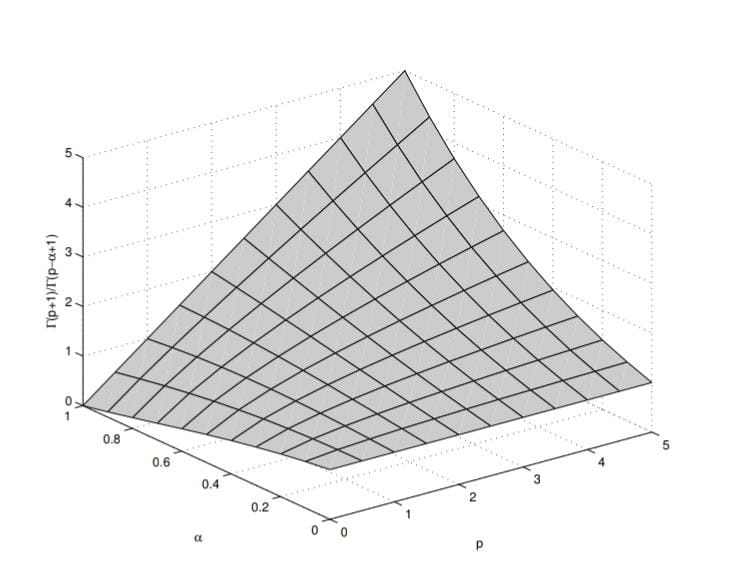
\includegraphics[scale=0.6]{The Coefficients in the derivative of the power function}
    \caption{The Coefficients in the derivative of the power function}
    \label{fig:5.1}
\end{figure}
\begin{exmp}
Suppose that $\alpha \in \mathbb{R}$ but $\alpha \notin \mathbb{N}$ ( $\alpha$ is the order of differentiation). Two examples are considered, namely fractional derivatives of the functions $t^{2}$ and $t$, i.e., $p=2$ and $p=1$ respectively. More examples are given in Appendix A.  
\end{exmp}
$\underline{p=2}$\\
Here, the function $t^{2}$ is discussed. Suppose that $0<\alpha<1$. Following (\ref{eq:5.3}) the fractional derivative is given in the following manner
$$
D_{*}^{\alpha} t^{2}=\frac{\Gamma(2+1)}{\Gamma(2-\alpha+1)} t^{2-\alpha}=\frac{2}{\Gamma(3-\alpha)} t^{2-\alpha}, n-1<\alpha<n<3 .
$$
More special cases can be considered for fixed values of the paramter $\alpha$, for example, $\alpha=1 / 3, \alpha=1 / 2$ and $\alpha=3 / 4$.\\
For $$\alpha=1 / 3 \quad D_{*}^{1 / 3} t^{2}=\frac{2}{\Gamma(3-1 / 3)} t^{2-1 / 3}=\frac{2}{\Gamma(8 / 3)} t^{5 / 3} \approx 1.33 t^{5 / 3},$$
for $$\alpha=1 / 2 \quad D_{*}^{1 / 2} t^{2}=\frac{2}{\Gamma(3-1 / 2)} t^{2-1 / 2}=\frac{8}{3 \sqrt{\pi}} \sqrt{t^{3}} \quad \approx 1.5 \sqrt{t^{3}},$$
for $$\alpha=3 / 4 \quad D_{*}^{3 / 4} t^{2}=\frac{2}{\Gamma(3-3 / 4)} t^{2-3 / 4}=\frac{2}{\Gamma(9 / 4)} t^{5 / 4} \approx 1.77 t^{5 / 4}.$$
These results are illustrated in Fig.(5.2). The graphs of the fractional derivatives are enclosed by the graphs of the classical integer-order derivatives everywhere except for a small interval. The greater the order of the derivative, the closer is its graph to the graph of the $1^{\text {st }}$ derivative of $t^{2}$, the smaller the order, the closer is its graph to the graph of the 0 -th derivative of $t^{2}$ (see also Remark 5.2.5).\\
\begin{figure}
    \centering
    \includegraphics[scale=0.6]{Fractional derivatives of f(t)=t^{2}}
    \caption{Fractional derivatives of $f(t)=t^{2}$}
    \label{fig:5.2}
\end{figure}
\begin{rmk}
Using $\Gamma(2)=1, \Gamma(3)=2$ (see (\ref{eq:8})) the following conclusion can be drawn
$$
D_{*}^{\alpha} t^{2}=\frac{2}{\Gamma(3-\alpha)} t^{2-\alpha} \rightarrow\left\{\begin{array}{l}
2 t, \alpha \rightarrow 1 \\
t^{2}, \alpha \rightarrow 0
\end{array}\right.
$$
which confirms the interpolation property (\ref{eq:4.7}) of the Caputo fractional derivative.
\end{rmk}
$\underline{p=1}$\\
Now $f(t)=t^{p}=t$. For this case (\ref{eq:5.3}) reads
$$
D_{*}^{\alpha} t=\frac{\Gamma(1+1)}{\Gamma(1-\alpha+1)} t^{1-\alpha}=\frac{1}{\Gamma(2-\alpha)} t^{1-\alpha} .
$$
Thus, for $\alpha=1 / 2$
$$
D_{*}^{1 / 2} t=\frac{1}{\Gamma(2-1 / 2)} t^{1-1 / 2}=\frac{2 \sqrt{t}}{\sqrt{\pi}},
$$
which coincides with formula (\ref{eq:4.2})
\par Some graphs can be seen in Fig. (5.3). Here the graphs of the fractional derivatives are enclosed between the graphs of the integer-order derivatives (except for a small interval). Although there is no convergence to the first derivative in the point 0 , the interpolation property still holds, since the fractional derivatives are defined only for $t>0$ (see Definition (4.1.1) and Remark 4.1.2).\\
\begin{figure}
    \centering
    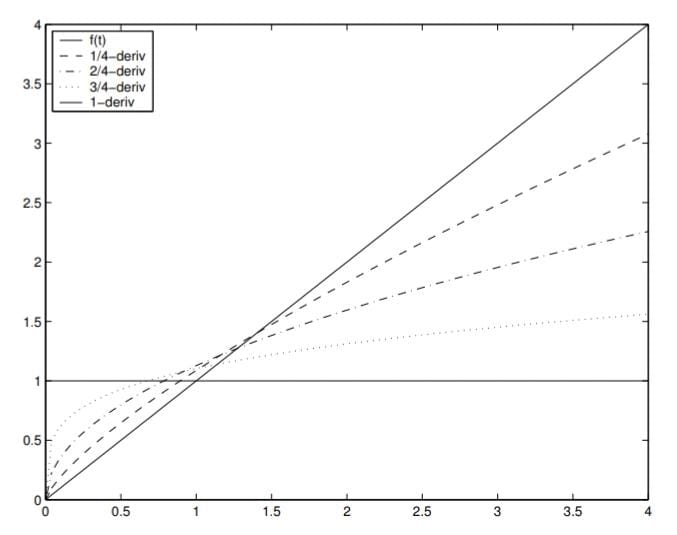
\includegraphics[scale=0.6]{Fractional derivatives of f(t)=t}
    \caption{Fractional derivatives of f(t)=t}
    \label{fig:5.3}
\end{figure}
In Fig. (5.4) a three dimensional graph of the fractional derivatives of the function $t^{2}$ is presented. Derivatives of order between 0 and 2 are considered. The bold lines are the classical integer-order derivatives, i.e., the functions $t^{2}, 2 t$ and 2 respectively. The fractional derivatives are interpolating these classical derivatives. The same figure can also be considered as a graph of the fractional derivatives of the function $t$, (more precisely, of the function $2 t$ ) of order between 0 and 1 , where the corresponding order for the function $t^{2}$ is between 1 and 2 , since $\left(t^{2}\right)^{\prime}=2 t$ and $D_{*}^{\alpha} t^{2}=D_{*}^{\alpha-1}\left(t^{2}\right)^{\prime}$ (see section 4.2).
\begin{figure}
    \centering
    \includegraphics[scale=0.6]{3D representation of the fractional derivatives of f(t)=t^{2}}
    \caption{3D representation of the fractional derivatives of $f(t)=t^{2}$}
    \label{fig:5.4}
\end{figure}
\section{The Exponential Function}
After discussing the fractional derivatives of the power function, we consider the exponential function $e^{\lambda t}$. The application of the Caputo operator is shown in the following statement.
\begin{thm}
Let $\alpha \in \mathbb{R}, n-1<\alpha<n, n \in \mathbb{N}, \lambda \in \mathbb{C}$. Then the Caputo fractional derivative of the exponential function has the form
\begin{equation}\label{eq:5.4}
D_{*}^{\alpha} e^{\lambda t}=\sum_{k=0}^{\infty} \frac{\lambda^{k+n} t^{k+n-\alpha}}{\Gamma(k+1+n-\alpha)}=\lambda^{n} t^{n-\alpha} E_{1, n-\alpha+1}(\lambda t),
\end{equation}
where $E_{\alpha, \beta}(z)$ is the two-parameter function of Mittag-Leffler type.
\end{thm}
\begin{proof}
To prove the theorem the relation between Caputo and Riemann-Liouville fractional derivatives (\ref{eq:4.24}) as well as the well-known Riemann-Liouville fractional derivative of the exponential function, namely,
$$
D^{\alpha} e^{\lambda t}=t^{-\alpha} E_{1,1-\alpha}(\lambda t)
$$
could be used. Then for the Caputo fractional derivative holds
$$
\begin{aligned}
D_{*}^{\alpha} e^{\lambda t} &=D^{\alpha} e^{\lambda t}-\sum_{k=0}^{n-1} \frac{t^{k-\alpha}}{\Gamma(k+1-\alpha)}\left(e^{\lambda t}\right)^{(k)}(0) \\
&=t^{-\alpha} E_{1,1-\alpha}(\lambda t)-\sum_{k=0}^{n-1} \frac{t^{k-\alpha}}{\Gamma(k+1-\alpha)} \cdot \lambda^{k} \\
&=\sum_{k=0}^{\infty} \frac{(\lambda t)^{k} t^{-\alpha}}{\Gamma(k+1-\alpha)}-\sum_{k=0}^{n-1} \frac{\lambda^{k} t^{k-\alpha}}{\Gamma(k+1-\alpha)} \\
&=\sum_{k=n}^{\infty} \frac{\lambda^{k} t^{k-\alpha}}{\Gamma(k+1-\alpha)} \\
&=\sum_{k=0}^{\infty} \frac{\lambda^{k+n} t^{k+n-\alpha}}{\Gamma(k+n+1-\alpha)} \\
&=\lambda^{n} t^{n-\alpha} E_{1, n-\alpha+1}(\lambda t)
\end{aligned}
$$
\end{proof}
Formula (\ref{eq:5.4}) matches the corresponding result, mentioned by Diethelm, Ford, Freed, and Luchko \cite{bb15} without any proof.\\
\ding{118} \quad \textbf{Special case}\\
Let $\lambda=$ 1. In Fig.(5.5) and Fig.(5.6) some graphs of fractional derivatives of the function $e^{t}$ are presented. The fractional derivatives are enclosed by the functions $e^{t}$ and $e^{t}-1$ and in general the exponential function and its derivatives have the same shape.
\par Inspecting (\ref{eq:5.4}) for $\lambda=1$ the right hand side doesn't dependent on $n$ but on $n-\alpha$. From this the following conclusion can be drawn.
\begin{prop}
Let $n-1<\alpha<n$ and $s \in \mathbb{Z}, s>-n$. Then
$$
D_{*}^{\alpha} e^{t}=D_{*}^{\alpha+s} e^{t} .
$$
This means in fact that for computing the Caputo fractional derivative of the exponential function only the value after the decimal point of the order of differentiation is important.
\end{prop}
\begin{figure}
    \centering
    \includegraphics[scale=0.6]{$0.5$-th and $2.8$-th fractional derivatives of $f(t)=e^{t}$ in the interval $(0,1.5]$}
    \caption{$0.5$-th and $2.8$-th fractional derivatives of $f(t)=e^{t}$ in the interval $(0,1.5]$}
    \label{fig:5.5}
\end{figure}
For example, for $\alpha=0.8, \alpha=1.8$ and $\alpha=7.8$ the same result is obtained, namely, $D_{*}^{0.8} e^{t}=D_{*}^{1.8} e^{t}=D_{*}^{7.8} e^{t}=\sqrt[5]{t} E_{1,1.2}(t).$
\par In addition, the $\alpha$-th order $(n-1<\alpha<n)$ fractional derivatives of the exponential function are \enquote{moving} from $e^{t}-1$ to $e^{t}$, for $\alpha$ taking values from $n-1$ to $n$. The same graphs are received for each $n \in \mathbb{N}$.
\par By using (\ref{eq:5.4}), the limits 
$$\lim_{\alpha \rightarrow n} D{*}^{\alpha} e^{t}$$ 
and $$\lim_{\alpha \rightarrow n-1} D_{*}^{\alpha} e^{t}$$ can be evaluated exactly 
$$\lim_{\alpha \rightarrow n} D_{*}^{\alpha} e^{t}=\lim_{\alpha \rightarrow n} t^{n-\alpha} E_{1, n-\alpha+1}(t)=E_{1,1}(t)=e^{t}=D^{n} e^{t}, n \in \mathbb{N},$$
$$
\begin{aligned}
\lim_{\alpha \rightarrow n-1} D{*}^{\alpha} e^{t} &=\lim_{\alpha \rightarrow n-1} t^{n-\alpha} E_{1, n-\alpha+1}(t)=t E_{1,2}(t) \\
&=t \sum_{k=0}^{\infty} \frac{t^{k}}{\Gamma(k+2)}=\sum_{k=0}^{\infty} \frac{t^{k+1}}{\Gamma(k+2)}=\sum_{k=1}^{\infty} \frac{t^{k}}{\Gamma(k+1)} \\
&=e^{t}-1=D^{n} e^{t}-\left.D^{n} e^{t}\right|_{t=0}, \quad n \in \mathbb{N} .
\end{aligned}
$$
These limit evaluations coincide with the interpolation property (\ref{eq:4.7}) of the Caputo derivative.
\begin{figure}
    \centering
    \includegraphics[scale=0.6]{$0.5$-th and $2.8$-th fractional derivatives of $f(t)=e^{t}$ in the interval $(0,3]$}
    \caption{$0.5$-th and $2.8$-th fractional derivatives of $f(t)=e^{t}$ in the interval $(0,3]$}
    \label{fig:5.6}
\end{figure}
\par In Fig.(5.7) a three-dimensional graph of the fractional derivatives of the function $e^{t}$ is presented. The left bold line is the function $e^{t}$ itself (which coincides with all its integer-order derivatives); the right bold line is the function $e^{t}-1$. In this figure the above results can be observed.

\section{Other Frequently Used Functions}
Another two functions that appear very often are the sine and the cosine functions. The behavior of the Caputo derivative applied to each of them is discussed in this section. Similar representations are given by Diethelm, Ford, Freed, and Luchko \cite{bb15}, which are also mentioned here for comparison.
\begin{thm}
Let $\lambda \in \mathbb{C}, \alpha \in \mathbb{R}, n \in \mathbb{N}, n-1<\alpha<n$. Then
\begin{equation}\label{eq:5.5}
D_{*}^{\alpha} \sin \lambda t=-\frac{1}{2} i(i \lambda)^{n} t^{n-\alpha}\left(E_{1, n-\alpha+1}(i \lambda t)-(-1)^{n} E_{1, n-\alpha+1}(-i \lambda t)\right) .
\end{equation}
\end{thm}
\begin{figure}
    \centering
    \includegraphics[scale=0.6]{3D representation of the fractional derivatives of $f(t)=e^{t}$}
    \caption{3D representation of the fractional derivatives of $f(t)=e^{t}$}
    \label{fig:5.7}
\end{figure}
\begin{proof}
The following representation of the sine function is used
$$
\sin z=\frac{e^{i z}-e^{-i z}}{2 i}, \quad z \in \mathbb{C} .
$$
Now, using the linearity property (4.2.3) of the Caputo fractional derivative and formula (\ref{eq:5.4}) for the exponential function it can be shown that
$$
\begin{aligned}
D_{*}^{\alpha} \sin \lambda t &=D_{*}^{\alpha} \frac{e^{i \lambda t}-e^{-i \lambda t}}{2 i} \\
&=\frac{1}{2 i}\left(D_{*}^{\alpha} e^{i \lambda t}-D_{*}^{\alpha} e^{-i \lambda t}\right) \\
&=\frac{1}{2 i}\left((i \lambda)^{n} t^{n-\alpha} E_{1, n-\alpha+1}(i \lambda t)-(-i \lambda)^{n} t^{n-\alpha} E_{1, n-\alpha+1}(-i \lambda t)\right) \\
&=-\frac{1}{2} i(i \lambda)^{n} t^{n-\alpha}\left(E_{1, n-\alpha+1}(i \lambda t)-(-1)^{n} E_{1, n-\alpha+1}(-i \lambda t)\right) .
\end{aligned}
$$
\end{proof}
In the same manner a formula for the Caputo derivative of the cosine function is received. The corresponding representation is
$$
\cos z=\frac{e^{i z}+e^{-i z}}{2}, \quad z \in \mathbb{C} .
$$
The corresponding result for the cosine function is formulated in the following statement.

\begin{thm}
Let $\lambda \in \mathbb{C}, \alpha \in \mathbb{R}, n \in \mathbb{N}, n-1<\alpha<n$. Then
\begin{equation}\label{eq:5.6}
D_{*}^{\alpha} \cos \lambda t=\frac{1}{2}(i \lambda)^{n} t^{n-\alpha}\left(E_{1, n-\alpha+1}(i \lambda t)+(-1)^{n} E_{1, n-\alpha+1}(-i \lambda t)\right) .
\end{equation}
\end{thm}
There exist representations of the Caputo derivative of the sine and cosine function in terms of the confluent hypergeometric function (Diethelm, Ford, Freed, and Luchko \cite{bb15}).
\par Let $\lambda, \alpha \in \mathbb{R}, n \in \mathbb{N}, n-1<\alpha<n$. Then
\begin{equation}\label{eq:5.7}
D_{*}^{\alpha} \sin \lambda t=\left\{\begin{array}{c}
-\frac{i \lambda^{n}(-1)^{n / 2} t^{n-\alpha}}{2 \Gamma(n-\alpha+1)}\left[{ }_{1}F_{1}(1, n-\alpha+1 ; i \lambda t)-{ }_{1} F_{1}(1, n-\alpha+1 ;-i \lambda t)\right],\\ \hfill \text{if $n$ is even,} \\
\frac{\lambda^{n}(-1)^{(n-1) / 2} t^{n-\alpha}}{2 \Gamma(n-\alpha+1)}\left[{ }_{1} F_{1}(1, n-\alpha+1 ; i \lambda t)+{ }_{1} F_{1}(1, n-\alpha+1 ;-i \lambda t)\right], \\ \hfill \text { if } n \text { is odd} . \\
\end{array}\right.
\end{equation}
and
\begin{equation}\label{eq:5.8}
D_{*}^{\alpha} \cos \lambda t=\left\{\begin{array}{l}
\frac{\lambda^{n}(-1)^{n / 2} t^{n-\alpha}}{2 \Gamma(n-\alpha+1)}\left[{ }_{1} F_{1}(1, n-\alpha+1 ; i \lambda t)+{ }_{1} F_{1}(1, n-\alpha+1 ;-i \lambda t)\right], \\ \hfill \text{if $n$ is even,} \\
\frac{i \lambda^{n}(-1)^{(n-1) / 2} t^{n-\alpha}}{2 \Gamma(n-\alpha+1)}\left[{}_{1} F_{1}(1, n-\alpha+1 ; i \lambda t)-{ }_{1} F_{1}(1, n-\alpha+1 ;-i \lambda t)\right], \\ \hfill \text { if } n \text { is odd} .\\
\end{array}\right.
\end{equation}
In this survey the representations (\ref{eq:5.5}) and (\ref{eq:5.6}) are preferred, since the Mittag-Leffler function is considered as a basic function of the fractional calculus.

All the main results from chapter 5 are summarized in table (5.1) The conditions for which these formulas hold are not given in the table for simplicity but can be found within chapter 5
}
\end{flushleft}
\end{center}

\newpage
    \begin{landscape}% Landscape page
    \section{Table for Caputo Derivatives of the most used functions}
        \centering % Center table
        \begin{center}
        \begin{tabular}{|m{5cm}|m{4.5cm}|m{16cm}|}
        \hline
        \hspace{1.5cm} \textbf{Function} & \hspace{2cm}$\bm{f(t)}$ & \hspace{5cm}\textbf{Caputo derivative} $\bm{D_{*}^{\alpha} f(t)}$\\
        \hline
         \hspace{0.5cm}Constant Function &\hspace{0.5cm} $f(t)=c=const $ &\hspace{6.5cm} $\mathbf{D}_{*}^{\alpha} c= 0 $ \\
        \hline
        \hspace{0.9cm}Power Function &\hspace{1cm} $ f(t)= t^{p}$ &\hspace{0.5cm} \begin{equation*} D_{*}^{\alpha} t^{p}=\left\{\begin{array}{ll} \frac{\Gamma(p+1)}{\Gamma(p-\alpha+1)} t^{p-\alpha}=D^{\alpha} t^{p}, & n-1<\alpha<n, p>n-1, p \in \mathbb{R}, \\ \\  0, & n-1<\alpha<n, p \leq n-1, p \in \mathbb{N} .\end{array}\right.\end{equation*}\\
        \hline
        \hspace{0.1cm} Exponential Function &\hspace{1cm} $ f(t)=e^{\lambda t}$ & 
        \begin{equation*}
D_{*}^{\alpha} e^{\lambda t}=\sum_{k=0}^{\infty} \frac{\lambda^{k+n} t^{k+n-\alpha}}{\Gamma(k+1+n-\alpha)}=\lambda^{n} t^{n-\alpha} E_{1, n-\alpha+1}(\lambda t)
\end{equation*} \\
        \hline
      \hspace{0.8cm}Sine Function & \hspace{0.8cm}$f(t)= \sin \lambda t $ & $
D_{*}^{\alpha} \sin \lambda t=-\frac{1}{2} i(i \lambda)^{n} t^{n-\alpha}\left(E_{1, n-\alpha+1}(i \lambda t)-(-1)^{n} E_{1, n-\alpha+1}(-i \lambda t)\right) 
$ \\ 
      \hline
      \hspace{0.7cm}Cosine Function &\hspace{0.8cm}$f(t)= \cos \lambda t $  &$
D_{*}^{\alpha} \cos \lambda t=\frac{1}{2}(i \lambda)^{n} t^{n-\alpha}\left(E_{1, n-\alpha+1}(i \lambda t)+(-1)^{n} E_{1, n-\alpha+1}(-i \lambda t)\right) 
$ \\
      \hline
        \end{tabular}
        \captionof{table}{\large{Caputo derivatives of the most used functions}}% Add 'table' caption
        \end{center}
         \newpage
        \addcontentsline{toc}{section}{\textbf{\Large{Appendix A : Table of Caputo derivative}}}
        \pagestyle{plain}
    \appendix
    \Large{\textbf{ Appendix A : Table of Caputo derivative}}
        \centering
        \begin{center}
        \Large{
        \setlength{\extrarowheight}{10pt}
        \begin{tabular}{|c|c|c|c|c|c|c|}
        \hline
         & $\bm{D_{*}^{\alpha} f(t)}$ & $\bm{D_{*}^{1/3} f(t)}$ & $\bm{D_{*}^{1/2} f(t)}$ & $\bm{D_{*}^{1/2} D_{*}^{1/2} f(t)}$ & $\bm{D_{*}^{1/2} D_{*}^{1/2} D_{*}^{1/2} f(t)}$ & $\bm{D_{*}^{1/2} D_{*}^{1/2} D_{*}^{1/2} D_{*}^{1/2} f(t)}$ \\
        \hline
        $ f(t) = const$ & 0 & 0 & 0 & 0 & 0 & 0 \\
        \hline
        $ f(t)=t $ & $\frac{1}{\Gamma(2-\alpha)} t^{1-\alpha} $ & $1.1077 t^{2/3}$ & $1.1284 t^{1/2}$ & $1 $ & $0$ & $0$\\
        \hline
        $ f(t)=t^{2} $ & $\frac{2}{\Gamma (3 - \alpha)} t^{2 -\alpha}$ & $1.3293 t^{5/3}$ & $1.5045 t^{3/2}$ & $2t$ & $2.2568 t^{1/2}$ & 2 \\
        \hline
      $ f(t)=t^{3} $ & $\frac{6}{\Gamma (4 - \alpha)} t^{3 -\alpha}$ & $1.4954 t^{8/3}$ & $1.8054 t^{5/2}$ & $3t^{2}$ & 4.5135 $t^{3/2}$ & $6t$ \\
      \hline
      $ f(t)=t^{4} $ & $\frac{24}{\Gamma (5 - \alpha)} t^{4 -\alpha}$ & $1.6314 t^{11/3}$ & $2.0633 t^{7/2}$ & $4t^{3}$ & $7.2216 t^{5/2}$ & $12t^{2}$ \\
      \hline
      $ f(t)=t^{5} $ & $\frac{120}{\Gamma (6 - \alpha)} t^{5 -\alpha}$ & $1.7479 t^{14/3}$ & $2.2926 t^{9/2}$ & $5t^{4}$ & $10.3166 t^{7/2}$& $20t^{3}$ \\
      \hline
      $ f(t)=t^{1/2} $ & $\frac{\sqrt{\pi}}{2\Gamma (3/2 - \alpha)} t^{1/2 -\alpha}$ & $0.9553 t^{1/6}$& 0.8862 & 0 & 0 & 0 \\
      \hline
      $ f(t)=t^{3/2} $ & $\frac{3\sqrt{\pi}}{4\Gamma (5/2 - \alpha)} t^{3/2 -\alpha}$ & $1.2282 t^{7/6}$& $1.3292 t$ & $1.5t^{1/2}$ & 1.3293 & 0 \\
      \hline
      $ f(t)=e^{t} $ &$t^{n-\alpha} E_{1, n-\alpha+1} (t)$ & $t^{2/3} E_{1,5/3} (t)$ & $t^{1/2} E_{1,3/2} (t)$  & $e^{t}$ & $t^{1/2} E_{1,5/3}(t)$ & $e^{t}$\\
      \hline
        \end{tabular}}
        \captionof{table}{Caputo derivatives of particular functions}% Add 'table' caption
        \end{center}
        \end{landscape}
    
    \thispagestyle{plain}
    
    \newpage
         \begin{center}
\justify
\Large{
\begin{thebibliography}{99} \addcontentsline{toc}{section}{\textbf{\Large{Bibliography}}}
\bibitem{bb1}Leibniz, G. W., 1695a. Letter from Hanover, Germany, to G. F. A. L'Hopital,
September 30, 1695, in Mathematische Schriften, 1849; reprinted 1962, Olms Verag,
Hidesheim, Germany, 2, 301-302
\bibitem{bb2}Leibniz, G. W., 1697. Letter from Hanover, Germany, to John Wallis, May 28 , 1697, in Mathematische Schriften; reprinted 1962, Olms Verag, Hidesheim,
Germany, 4, 25 .
\bibitem{bb3}Euler, L., 1738. De progressionibus transcendentibus, sev quarum termini generales algebraice dari nequent, Commentarii Academiae Scientiarum Imperialis
Scientiarum Petropolitanae, 5, p. $55 .$
\bibitem{bb4}Fourier, J. B. J., 1822, Theorie analytique de la chaleur, Oeuvres de Fourier, Vol. 1, Firmin Didot, Paris, p. $508 .$
\bibitem{bb5}Liouville, J., 1834. Memoire sur le theoreme des fonctions complementaraires, $J$. Reine Angew. Math. (Crelle's J.), 11, 1-19.
\bibitem{bb6} De Morgan, A., 1840. The Differential and Integral Calculus Combining Differentiation, Integration, Development, Differential Equations, Differences, Summation, Calculus of Variations...with Applications to Algebra, Plane and Solid Geometry, Baldwin and Craddock, London; published in 25 parts under the superintendence of the Society for the Diffusion of Useful Knowledge, pp. 597-599. 
\bibitem{bb7} Center, W., 1848. On the value of $(\mathrm{d} / \mathrm{dx})^{\theta} \mathrm{x}^{0}$ when $\theta$ is a positive proper fraction, Cambridge Dublin Math. J., 3, 163-169.
\bibitem{bb8} Cayley, A., 1990. Note on Riemann's paper, Math. Ann., 16, 81-82.
16
\bibitem{bb9} Davis, H. T., 1927. The application of fractional operators to functional equations, Amer. J. Math., 1936, V49, 123-142.
\bibitem{bb10} Miller, Kenneth, S, and Ross, Bertram, 1993. An Introduction to the Fractional Calculus and Fractional Differential Equations, John Wiley \& Sons, Inc. pp. 1 to $20 .$
\bibitem{bb11} John M. Beach, Rowan University, Fractional Derivatives ( Thesis ) \url{https://rdw.rowan.edu/etd/1630/} %Used For History of Fractional Derivatives 
\bibitem{bb12} Joseph M. Kimeu, Western Kentucky University, Fractional Calculus: Definitions and Applications ( Thesis ) \\
\url{https://digitalcommons.wku.edu/theses/115/} %Used For Mittag-Leffler Function
\bibitem{bb13} Caputo M., Linear model of dissipation whose $Q$ is almost frequency independent - $I I$, The Geophysical Journal of the Royal Astronomical Society, Vol. 13, 1967, 529-539.
\bibitem{bb14}Debnath L., Fractional integral and fractional differential equations in fluid mechanics, Fractional Calculus and Applied Analysis, Vol. 6, No. 2, 2003, 119-155.
\bibitem{bb15} Diethelm K., Ford N. J., Freed A. D., and Luchko Yu., Algorithms for the fractional calculus: a selection of numerical methods, Preprint submitted to Computer Methods in Applied Mechanics and Engineering, 17 March, $2003 .$
\bibitem{bb16}Gradshteyn I. and Ryzhik I., Table of integrals, series, and products, Academic Press, New York, $1980 .$
[Originally published in Russian, Tablitsy integralov, summ, ryadov i proizvodeniy, Gosudarstvennoe Izdatel'stvo Fiziko-Matematicheskoy Literatury, Moscow, 1963.]
\bibitem{bb17}Greenberg M., Foundations of applied mathematics, Prentice-Hall Inc., Englewood Cliffs, N.J. 07632, 1978 .
\bibitem{bb18}Gorenflo R. and Mainardi F., Essentials of fractional calculus, Preprint submitted to MaPhySto Center, January 28, $2000 .$
\bibitem{bb19}Miller K. and Ross B., An introduction to the fractional calculus and fractional differential Equations, John Wiley \& Sons Inc., New York, $1993.$
\bibitem{bb20} Moshrefi-Torbati M. and Hammond J. K., Physical and geometrical interpretation of fractional operators, Elsevier Science, Great Britain, $1998 .$
\bibitem{bb21}Oldham K. and Spanier J., The fractional calculus, Academic Press, New York London, $1974 .$
\bibitem{bb22}Podlubny I., Fractional differential equations, Academic Press, San Diego, 1999
\bibitem{bb23}Podlubny I., Geometric and physical interpretation of fractional integration and fractional differentiation, Fractional Calculus and Applied Analysis, Vol. 5, 2002, 367386.
\bibitem{bb24}Samko S., Kilbas A., and Marichev O., Fractional integrals and derivatives. Theory of applications, Gordon and Breach Science Publishers, Amsterdam, $1993 .$
[Originally published in Russian, Integrals and derivatives of fractional order and some of their applications, Nauka i Tekhnika, Minsk, 1987.]
\bibitem{bb25}Mariya Kamenova Ishteva, University Karlsruhe from Sofia (Bulgaria), Properties and Applications of the Caputo Fractional Operator, February 2005 ( Thesis )\\
%Used For Caputo Derivative and Examples of Fractional Derivative
\end{thebibliography}}
       \end{center}

\end{document}